%-----------------------------------------------------------------------------------------
%  Dieses Projekt wurde erstellt mit der LaTeX Vorlage von Jonas Bingel
%  Die LaTeX Vorlage kann heruntergeladen werden unter: github.com/JonasBingel/HSMZ-Thesis-Template
% -----------------------------------------------------------------------------------------

% Erklärender Text zu dieser Datei --------------------------------------------------------
% Die Datei Arbeit.tex ist die Hauptdatei, die dem LaTeX-Kompiler übergeben wird.
% Diese Datei ist zu verwenden, wenn die eigentliche Haus/Bachelor/Masterarbeit erstellt werden soll.
% In dieser Datei wird
%  - das Dokument erstellt und alle anderen tex-Dateien werden geladen.
%  - die .bib-Datei eingebunden zur Bereitstellung der Quellen
%  - die Struktur des Dokuments wird definiert
% -----------------------------------------------------------------------------------------

\documentclass[
% ngerman, % neue Deutsche Rechtschreibung
headings=normal, % normale Headings
captions=tableheading, % Positioniert Captions über Tabellen
numbers=noenddot, % Keine Punkte hinter Kapiteln, Sektionen, Abbildungen, etc.
listof=totoc,
bibliography=totoc,
%usegeometry, % Auskommentieren wenn Package geometery verwendet wird
%overfullrule, % entfernen nach abschluss der bearbeitung
final,
% Default Values, die scrreprt nutzt
oneside, % Einseitige Seitengenerierung
12pt, % Font size
a4paper, % paper
]{scrreprt}
\linespread{1.5}
\KOMAoptions{%
  DIV=12,
  parskip=half*,
  %BCOR=3mm, % absoluter Wert der Bindekorrektur
}

% Erklärender Text zu dieser Datei --------------------------------------------------------
% Die Datei Metadaten.tex dient der Definition von Metadaten zur vorliegenden Arbeit.
% Dies umfasst Informationen zu
%  - der Arbeit selbst(Titel, Art)
%  - dem Betreuer
%  - dem Hochschule
%  - ggf. kooperierenden Unternehmen
% Die Metadaten werden genutzt in Titelseite.tex, Sperrvermerk.tex und Erklaerung.tex
% Ferner werden die Metadaten des exportierten PDFs entsprechend gesetzt - eine Konfiguration ist in Packages.tex möglich.
% -----------------------------------------------------------------------------------------

% Meta-Daten zu dieser Arbeit ------------------------------------------------------------
\newcommand{\art}{Masterarbeit\xspace}
\newcommand{\titel}{Sensorama: A task-specific Telepresence Application for Contemporary Dance\xspace}
\newcommand{\hochschule}{Hochschule Mainz}
\newcommand{\hochschulezusatz}{University of Applied Sciences}
\newcommand{\logo}{logo_hsmz}
\newcommand{\fachbereich}{Technik}
\newcommand{\fachrichtung}{Geoinformatik und Vermessung}
\newcommand{\studiengang}{berufsbegleitenden Masterstudiengang Geoinformatik}
\newcommand{\akadGrad}{Master of Engineering}

\newcommand{\autor}{Anton Koch}
\newcommand{\strasseAutor}{}
\newcommand{\stadtAutor}{}
\newcommand{\matrikelnr}{946750}
\newcommand{\standnummer}{268}

\newcommand{\unternehmen}{Unternehmen}
\newcommand{\datumAblaufSperrvermerk}{01.01.1970}

\newcommand{\betreuer}{Prof. Dr. Pascal Neis}
\newcommand{\datumAbgabe}{14.02.2023}
\newcommand{\bearbeitungsZeitraum}{15.8.2023 bis 14.2.2024}
\newcommand{\ort}{Mainz}

% Erklärender Text zu dieser Datei --------------------------------------------------------
% Die Datei Packages.tex dient als zentrale Datei, in der alle genutzten Packages geladen und konfiguriert werden.
% Basierend auf den Anforderungen sind ggf. Konfigurationen vereinzelt zu ändern - entsprechende Stellen sind mit %TODO gekennzeichnet.
% Beispiele für solche Anforderungen sind
%  - Package biblatex: Definition, des Zitationsstils und Aufbau des Literaturverzeichnisses; Default ist IEEE, Konfiguration für APA ist hinterlegt
%  - Package minted: Definition, wie Source Code von Sprachen dargestellt werden soll
%  - Zur korrekten Darstellung des Inhaltsverzeichnisses die "breiteste" Seitenzahl angeben
%
% HINWEIS: Die Reihenfolge, in der Packages geladen werden ist wichtig. Hinweise aus den Dokumentationen der einzelnen Packages sind daher unbedingt zur berücksichtigen, wenn weitere Packages aufgenommen werden sollen.
% -----------------------------------------------------------------------------------------
% \usepackage[a4paper, top=2.5cm]{geometry}
\usepackage[utf8]{inputenc}
\usepackage[T1]{fontenc}
\usepackage[UKenglish]{babel}
\usepackage{lmodern}
\usepackage{fancyhdr}
\usepackage{xspace} % Leerzeichen hinter parameterlosen Makros nicht als Endzeichen interpretieren
\usepackage{graphicx} %Abbildungen
\usepackage{pdfpages} %Einfügen von PDF-Seiten
\usepackage[inkscapeformat=png]{svg} %Einfügen von SVG Grafiken
\includepdfset{scale=0.7, frame, pagecommand={\thispagestyle{plain}}}
\graphicspath{{04_Artefakte/01_Abbildungen/}}
\usepackage{caption} % Bildunterschriften
\usepackage{subcaption} % https://www.ctan.org/pkg/subcaption

\usepackage{tabularx} % Tabellen
\usepackage{booktabs} % Bessere Tabellen
\usepackage[longtable]{multirow}
\usepackage{longtable}
\usepackage{multicol}

\usepackage{amsmath}
\usepackage{amsfonts}
\usepackage{bbm}

\usepackage{xcolor}
%\usepackage{chngcntr} % fortlaufende Nummerierung von Fußnoten

\usepackage[colorinlistoftodos]{todonotes} % to disable todos use option disable, alternatively use obeyDraft or obeyFinal
\usepackage{blindtext}

\usepackage{microtype} % auskommentieren moeglich, wenn Typografie nicht zufriedenstellend

\usepackage[bottom]{footmisc} % https://golatex.de/viewtopic.php?f=21&t=24052
% Verlinkung und PDF Bookmarks https://tex.stackexchange.com/a/83051
\usepackage[nospace]{varioref}
% extensions keep all links black, only urls are blue: https://tex.stackexchange.com/a/401885/220502
\usepackage[hidelinks, colorlinks, allcolors=., urlcolor=blue]{hyperref}
\usepackage{bookmark}
\hypersetup{
    pdftitle={\titel},
    pdfauthor={\autor},
    pdfcreator={\autor},
    pdfsubject={\titel},
    pdfkeywords={\titel},
}
\usepackage{cleveref}

% Literaturverzeichnis und Quellenverwaltung mittels biblatex
%TODO Änderungen des Zitationsstils und Literaturverzeichnisses
% Zitationsstil hier auswählen:

\newcommand{\ZitatStil}{apa} % (apa oder ieee)

\ifthenelse{\equal{\ZitatStil}{apa}}{%
  \usepackage[sortlocale=auto,sorting=nyt,style=apa]{biblatex}%
}{
\ifthenelse{\equal{\ZitatStil}{iee}}{%
  \usepackage[backend=biber,style=ieee,dashed=false,]{biblatex}%
}}


% Verwalten von Abkuerzungen und einem Abkuerzungsverzeichnis
\usepackage[printonlyused]{acronym} % https://www.ctan.org/pkg/acronym

% Packages for forcing floats https://robjhyndman.com/hyndsight/latex-floats/
\usepackage{afterpage}
\usepackage[section]{placeins}
\usepackage{censor}


% Erstellen eines Symbolverzeichnisses
\usepackage[intoc, english, stdsubgroups]{nomencl} % https://www.ctan.org/pkg/nomencl
\usepackage{siunitx}
\newcommand{\nomunit}[1]{%
    \renewcommand{\nomentryend}{\hspace*{\fill}\si{#1}}}
\makenomenclature

%TODO Definition der Darstellung von Source Code
\usepackage[newfloat, cache]{minted} % https://www.ctan.org/pkg/minted
\SetupFloatingEnvironment{listing}{name=Listing, placement=b}
\SetupFloatingEnvironment{listing}{listname={Listingverzeichnis}}
\setminted[java]{linenos, fontsize=\footnotesize, frame=lines, breaklines, breakbefore={.}}
\setminted[python]{linenos, fontsize=\footnotesize, frame=lines, breaklines, breakbefore={.}}
\setminted[js]{linenos, fontsize=\footnotesize, frame=lines, breaklines, breakbefore={.}}
\setminted[json]{linenos, fontsize=\footnotesize, frame=lines, breaklines, breakbefore={.}}
\setminted[text]{fontsize=\footnotesize, frame=lines}
\usemintedstyle{friendly}
% new environment for listings longer than one page; https://tex.stackexchange.com/a/53540
\newenvironment{longlisting}{\captionsetup{type=listing}}{}
\usepackage{csquotes}


% Darstellung von Algorithmen und Pseudocode
% do NOT use option naturalnames if you compile with pdflatex and use hyperref
\usepackage[linesnumbered, commentsnumbered, ruled]{algorithm2e} 
\renewcommand{\listalgorithmcfname}{Algorithmusverzeichnis}
\addtotoclist[float]{loa}
\renewcommand\listofalgorithms{\listoftoc[{\listalgorithmcfname}]{loa}}
%\SetAlFnt{\small \normalfont \sffamily} 
\SetAlFnt{\footnotesize} 


% Erstellung neuer Verzeichnisse; Code weitgehend von Markus Kohm und komascript.de 
\DeclareNewTOC[%
  owner=anhang,
  listname={Appendix Listing},% Titel des Verzeichnisses
]{atoc}

\DeclareNewTOC[%
  type=equation,
  listname={Formelverzeichnis},
  tocentrynumwidth=2.3em,
]{loe}

\makeatletter
\renewcommand\@pnumwidth{2em} % vermeiden von overful hbox im Inhaltsverzeichnis

\AfterTOCHead[atoc]{\let\if@dynlist\if@tocleft}
\newcommand*{\useappendixtocs}{%
  \renewcommand*{\ext@toc}{atoc}%
  \scr@ifundefinedorrelax{hypersetup}{}{% damit es auch ohne hyperref funktioniert
    \hypersetup{bookmarkstype=atoc}%
  }%
}
\newcommand*{\usestandardtocs}{%
  \renewcommand*{\ext@toc}{toc}%
  \scr@ifundefinedorrelax{hypersetup}{}{% damit es auch ohne hyperref funktioniert
    \hypersetup{bookmarkstype=toc}%
  }%
  \renewcommand*{\ext@figure}{lof}%
  \renewcommand*{\ext@table}{lot}%
}
\scr@ifundefinedorrelax{ext@toc}{%
  \newcommand*{\ext@toc}{toc}
  \renewcommand{\addtocentrydefault}[3]{%
    \expandafter\tocbasic@addxcontentsline\expandafter{\ext@toc}{#1}{#2}{#3}%
  }
}{}
\newcommand*{\@currententry}{}
% Zwei amsmath-Anweisungen ändern:
\g@addto@macro\make@display@tag{\set@currententry}%
\def\tagform@#1{\maketag@@@{(\ignorespaces#1\unskip\@@italiccorr)}%
  \set@currententry}
\newcommand*{\set@currententry}{%
  \typeout{set current entry}%
  \ifx\@currententry\@empty\else
    \addcontentsline{loe}{equation}{\protect\numberline{\@currentlabel}%
      \@currententry}%
    \global\let\@currententry\@empty
  \fi
}
% Neue Benutzeranweisung
\newcommand*{\equationentry}[1]{%
  \gdef\@currententry{#1}%
}

\makeatother

\usepackage{xpatch}
\xapptocmd\appendix{%
  \useappendixtocs
  \pdfbookmark{Appendix}{appendix}
  \listofatocs
  \addcontentsline{toc}{chapter}{Appendix}
  \bookmarksetupnext{level=-1}
}{}{}

% Pakete, die fuer Informatik Sinn ergeben koennten
% \usepackage{bytefield} % illustration of fields of data https://www.ctan.org/pkg/bytefield


% Uebersetzung fuer Eintraege im Abkuerzungsverzeichnis - Code uebernommen von https://tex.stackexchange.com/a/135507
\makeatletter
\newcommand{\acroforeign}[1]{}

% patch the environment to print the foreign definition:
\AtBeginEnvironment{acronym}{%
  \def\acroforeign#1{ (#1)}%
}

% patch the acronym definition to safe the foreign definition:
\expandafter\patchcmd\csname AC@\AC@prefix{}@acro\endcsname
  {\begingroup}
  {\begingroup\def\acroforeign##1{\csdef{ac@#1@foreign}{##1, }}}
  {}
  {\fail}

% %   renew the first output to include the foreign definition if given:
\renewcommand*{\@acf}[2][\AC@linebreakpenalty]{%
  \ifAC@footnote
    \acsfont{\csname ac@#2@foreign\endcsname\AC@acs{#2}}%
    \footnote{\AC@placelabel{#2}\AC@acl{#2}{}}%
  \else
    \acffont{%
      \AC@placelabel{#2}\AC@acl{#2}%
      \nolinebreak[#1] %
      \acfsfont{(\acsfont{\csname ac@#2@foreign\endcsname\AC@acs{#2}})}%
    }%
  \fi
  \ifAC@starred\else\AC@logged{#2}\fi
}
\makeatother

% Adjusting the width that is reserved for the  pagenumber in listings
% https://projekte.dante.de/DanteFAQ/Verzeichnisse#2
% https://de.comp.text.tex.narkive.com/fAP3Znev/overfull-hbox-im-inhaltsverzeichnis
\makeatletter
\AtBeginDocument{
\newlength{\mylen}
\setlength{\mylen}{\widthof{XVIII}} %TODO hier Text eintragen, der der breitesten Seitennummer im Inhaltsverzeichnis oder einem der anderne Verzeichnisse entspricht
\renewcommand*\@pnumwidth{\the\mylen}
}
\makeatother

% Allow a chapter to occur without a headline to be able to cram both language abstracts on page
\makeatletter
\newcommand{\unchapter}[1]{%
  \begingroup
  \let\@makechapterhead\@gobble % make \@makechapterhead do nothing
  \chapter{#1}
  \endgroup
}
\makeatother

\input{00_Allgemein/Befehle}

% Typesetting options
\widowpenalty=10000     % Hurenkinder
\clubpenalty=10000      % Schusterjungen



\addbibresource{sample.bib}
\addbibresource{github_repositories.bib}
\addbibresource{surveys.bib}
\addbibresource{standards.bib}
% Wegen dem folgenden Befehl werden im Literaturverzeichnis alle Quellen gelistet, die in der .bib Datei enthalten sind.
% Wird der Befehl entfernt, werden nur die Quellen gelistet, die auch zitiert werden.
% Der Befehl sollte bei Abgabe der Bachelorarbeit entfernt werden.
% \nocite{*}
% \newcounter{romanConsecutive}

% Set ToC depth to subsubsection
% \setcounter{tocdepth}{4}
% \setcounter{secnumdepth}{4}

\begin{document}
\setlength{\aboverulesep}{0pt}
\setlength{\belowrulesep}{0pt}
% \setlength{\extrarowheight}{.75ex}

% \selectlanguage{ngerman}
\include{00_Allgemein/ToDo}

\pagestyle{empty}
\renewcommand*{\chapterpagestyle}{empty}
% Erklärender Text zu dieser Datei --------------------------------------------------------
% Die Datei 02_Titelseite.tex dient der Definition der Titelseite.
% Alle Angaben auf der Titelseite werden mit Informationen aus Metadaten.tex gefüllt
% Solange das Design der Titelseite nicht angepasst werden soll, sind in dieser Datei keine manuellen Änderungen notwendig.
% -----------------------------------------------------------------------------------------
\begin{titlepage}

\begin{minipage}{\textwidth}
		\noindent \hfill \includesvg{\logo}
\end{minipage}
\vspace{4em}

\begin{center}
    {\huge \art}

    {\Large zur Erlangung des akademischen Grades \akadGrad}\\
    {\Large im \studiengang}

    \vspace{4em}

    \textbf{{\Large \titel}}

    \vspace{4em}

    \hochschule \\
    Fachbereich \fachbereich \\
    Fachrichtung \fachrichtung

    \vspace{10em}

	\begin{multicols}{2}
	\begin{minipage}{\textwidth}
		\begin{tabbing}

		Vorgelegt von:  \hspace*{0.5em}\= \autor \\
		\> \strasseAutor \\
        \> \stadtAutor \\
        Matrikel-Nr.: \> \matrikelnr
        \end{tabbing}
    \end{minipage}
        
	\begin{minipage}{\textwidth}
		\begin{tabbing}
		 
        Betreut von: \hspace*{1.5em}\= \betreuer \\
        Eingereicht am: \> \datumAbgabe \\
        Studienort: \> \ort \\
        Standnummer: \> \standnummer
		\end{tabbing}

	\end{minipage}
	\end{multicols}
\end{center}
\end{titlepage}

% Erklärender Text zu dieser Datei --------------------------------------------------------
% Die Datei 03_Erklaerung.tex dient der Definition der Eidesstattlichen Erklärung.
% Die Datei enthält den Text, der im Leitfaden der Hochschule Mainz vorgegeben ist.
% Wenn ein Bild einer Unterschrift eingefügt werden soll, ist an der Stelle %TODO dem Hinweis zu folgen.
% -----------------------------------------------------------------------------------------
\pdfbookmark{Erklärung}{erklaerung}
\addchap*{Erklärung}
Hiermit erkläre ich, dass ich die vorliegende Masterarbeit
\begin{quote}
\textbf{\titel}   
\end{quote}

selbständig ohne fremde Hilfe angefertigt habe.
Ich habe nur die in der Arbeit ausdrücklich benannten Quellen und Hilfsmittel benutzt. 
Wörtlich oder sinngemäß übernommenes Gedankengut habe ich als solches kenntlich gemacht.

\vspace{6em}
%TODO Wenn eine Unterschrift eingefügt werden soll, muss nachfolgender Kommentar eingefügt werden
% Einfuegen der Unterschrift als Datei "signature.png", Scale muss ggf. angepasst werden
% \begin{figure}[h]
%     \hspace{9cm}
%     \includegraphics[scale=0.2]{04_Artefakte/01_Abbildungen/signature.png}
% \end{figure}
\ort, den \datumAbgabe \hfill \autor 


\pdfbookmark{Abstract}{abstract}
\section*{Abstract}

This study investigates the feasibility of creating a fully customised and task-specific telepresence application based exclusively on open web standards and free software for contemporary dance practice.
It surveys existing technologies and paradigms and establishes a reference implementation called \textquote{Sensorama} to evaluate basic functionality and the development process.
The existing technological landscape and the feasibility of producing task-specific web applications as an intrinsic component of interdisciplinary projects focusing on digital practice are positively assessed.
An alternative development strategy termed \textquote{code composting} is proposed and recommended for smaller creative projects, describing a process-oriented cyclical method of intuitive composition and analytical decomposition.

\textbf{Keywords:} telepresence, contemporary dance, motion capture, arts, open-source, computer science, software engineering


\section*{Kurzzusammenfassung}

Diese Studie untersucht die Machbarkeit der Entwicklung einer aufgabenspezifischen Telepräsenzanwendung für den Einsatz im zeitgenössischen Tanz und basierend auf offenen Standards.
Es wird ein Überblick über existente Technologien erabeitet und eine Referenzimplementierung names \textquote{Sensorama} erstellt, deren Entwicklungsprozess und abstrakte Funktion evaluiert wird.
Die technologischen Möglichkeiten und die Praktikabilität einer fallspezifischen Softwareimplementierung als Teil von interdisziplinären Projekten werden positiv bewertet.
Es wird der Begriff der \textquote{Code-Kompostierung} eingeführt, der sich als prozessorientierte Entwicklungsstrategie auf Zyklen intuitiver Komposition und analytischer Dekomposition stützt und für kleinere kreative Projekte zu empfohlen wird.
 
 \textbf{Schlagwörter:} Open-Source, Telepräsenz, Zeitgenössischer Tanz, Bewegungserfassung, Kunst, Informatik, Softwareentwicklung
 

\pagenumbering{arabic}
\pagestyle{fancy}
\fancyhf{}
\fancyheadoffset{0cm}
\renewcommand{\headrulewidth}{0pt}
\renewcommand{\footrulewidth}{0pt}
\fancyhead[R]{\thepage}
\fancypagestyle{plain}{
  \fancyhf{}
  \fancyhead[R]{\thepage}
}
% \pagestyle{plain}
\renewcommand*{\chapterpagestyle}{fancy}
% \pagenumbering{Roman}
\include{01_Vortext/05_Verzeichnisse}
\include{00_Allgemein/Nomenklatur}

% \setcounter{romanConsecutive}{\value{page}}
% \pagenumbering{arabic}
\chapter{Introduction}
\label{ch:introduction}

\section{Background}
\label{sec:background}

Remote collaboration has become increasingly prevalent in various professional environments through broader digitalisation efforts and significantly accelerated during the COVID-19 pandemic.
As a result, teleconferencing and telepresence platforms that were initially used primarily for international business relations are now much more common in many work environments.
These technologies allow people to work together remotely in real time, usually focusing on streaming video and audio, document sharing and collaborative whiteboarding.
While this covers most use cases in desk-based workplaces, it lacks the immersive qualities required for practices such as contemporary dance, where people relate to physical presence and shared space.
This became apparent in March 2020, when dancers could no longer rehearse and work together due to the lockdown.
Despite this, there were attempts at using videoconferencing to stream and record collaborative rehearsals or dance classes.
Still, these were confined to a screen-centric interface and limited to audio and video.

While commercial conferencing tools dominate in popularity among conferencing applications~\parencite{mostPopularConferencingPlatforms}, there are several free and open-source alternatives.
However, these all focus on the most basic form of screen-based conferencing.
Various domain-specific solutions for specialised applications, mainly in telemedicine, industry and the military, support more immersive remote collaboration.
Still, these are task-specific and difficult to afford for smaller creative or artistic project setups.

Support for web standards is driven by key industry players~\parencite{pushingInteroperabilityForward}, making a wide range of basic functionality accessible in web browsers, as well as access to display and sensor technology and cross-platform deployment on desktop and mobile devices.
This development now provides an increased potential for smaller and more task-specific applications to be built and deployed relatively quickly.
It opens up new possibilities for niche cases of remote collaboration, such as dance practice, where the collaborative agency could be extended from a composite of video streams to the creation of shared virtual environments that facilitate a more personal form of mediating a sense of shared presence.

The standard for \ac{RTC} in Browsers or \ac{WebRTC}~\parencite{webRtcSpec} was first proposed by Google in 2011 and became an official \ac{W3C} standard in 2021~\parencite{webRtcOfficialWebStandard}.
It has become the basis for numerous applications, such as some of the conferencing tools mentioned above, media streaming servers, or real-time frameworks.
In its most basic form, \ac{WebRTC} establishes peer-to-peer connections between devices, allowing low-latency exchange of media streams and arbitrary messages over data channels.
However, it can accommodate other more complex and versatile scenarios.

\section{Proposal}
\label{sec:proposal}

The proposed study examines the feasibility of creating a customised telepresence experience that explicitly covers a specific task not provided by common platforms or products.
A potential target audience for such an application would be tiny and hardly warrants a commercial strategy of external product development, marketing and support.
Extensive software development budgets are also rare in funding schemes supporting smaller cultural production endeavours, and it is relatively common for practitioners themselves to dabble in experimental development or to have a creative coder on the team.
To keep the budgetary requirements for such an implementation at a minimum, relying on open standards and non-proprietary components is imperative.
While the implementation has to fulfil a particular task, some level of abstraction, modular composition and separation of concerns are important design factors that allow for establishing a technological base that can be reused in multiple contexts with less work in subsequent deployment instances.

To support a broad range of scenarios, the application core should support the real-time streaming of any type of sensor data in addition to the usual video and audio streams.
This would allow augmenting the telepresence environment with spatial data, sensor readings or generative data sources.
The data could then be streamed as is but visualised, sonified, or otherwise analysed and processed on the receiving devices as required by the implemented use case.
In this reference implementation, movement sonification is implemented as an alternative to the visually-centred conferencing paradigms.
As movement in front of a screen or with headsets can be somewhat limiting, the idea is to use spatial audio for movement sonification and voice communication to provide a sense of positional orientation in relation to the virtual presence in the space.
Focused on a scenario of two participants moving at remote locations but in virtually overlayed spatial dimensions, this setup could enable exploration of moving together by attempting to achieve some form of acoustic harmony or rhythm to supplant an actual shared physical presence.
This implementation targets only a small audience in that it requires practice and a deep engagement with the sonification method, explained in detail in \autoref{sec:sonification-method-and-sound-spatialisation}, as it would be specifically built to express a specific style of movement that would not be intuitive for every potential user alike.
It should also be used by dancers with a shared experience of moving together so that verbal communication can support navigating a shared movement vocabulary and connecting to the memory of shared physical practice.
Creative design processes and user experience are deemed outside the scope of this study, as the focus lies on examining the general feasibility and affordability of using open standards and free software to enable the creation of a task-specific real-time application, exemplified by the proposed reference implementation and examined in its general abstract functionality instead of usability or user experience.

\section{Structural outline}
\label{sec:outline}

The study starts from a survey of \emph{conceptual foundations} presenting existing paradigms and technologies to support the development of web-based real-time applications (\autoref{ch:conceptualfoundations}), establishes a \emph{research methodology} (\autoref{ch:methodology}) and presents an \emph{application concept} (\autoref{ch:concept}) as well as a description of the resulting {reference implementation} (\autoref{ch:implementation}).
The reference implementation is the basis for a \emph{discussion} of the reference implementation's general performance, code quality, the amount of time invested in its creation and a critical reflection on the development process (\autoref{ch:discussion}).
The study \emph{concludes} with a general recommendation on the feasibility of creating such a \textquote{single-use} application for a specific task and an \emph{outlook} for future implications and possibilities resulting from this research (\autoref{ch:conclusion-and-outlook}).

\chapter{Conceptual foundations}
\label{ch:conceptualfoundations}

\section{Telepresence}
\label{sec:telepresence}

The term \emph{telepresence} first appears in an article by Marvin Minsky, roughly defined as a form of remote robotic operation, that \textquote{emphasises the importance of high‑quality sensory feedback} and the author posits that its realisation's biggest challenge is \textquote{achieving that sense of \textquote{being there.}}~\parencite{minskyTelepresence}.
Considering the general technological development at the time, Minsky argued from a standpoint concerned primarily with robotic manipulators that perform remote labour, enhancing the operator's physical abilities and safety.
Today, virtual and augmented reality, telepresence, and general presence research present much more diverse application scenarios.
While there are applications of remote robotic control in retail, industry, telemedicine and police or military, the most common instance has become the teleconferencing application relaying video and audio streams and allowing chat and collaborative whiteboards.

In this study, the term telepresence is used to explicitly describe a virtual or augmented environment that allows multiple people to experience some form of shared presence, immersion and interaction.
The concepts of \emph{presence} and \emph{immersion} require a precise contextualisation for this study.
The article~\textquote[\cite{surveyOfPresence}]{A Survey of Presence and Related Concepts} presents a wide range of possible variations and specific definitions for these concepts in different contexts and environments.
There, the authors state that presence \textquote{is most commonly defined as something akin to the feeling of \textquote{being there} in a virtual place}~\parencite[2]{surveyOfPresence} and immersion can be understood as \textquote{an objective characteristic of a [virtual environment] system} that, as the authors are citing Slater, \textquote{provides the boundaries within which [presence] can occur}~\parencite[3]{surveyOfPresence}.
In this study, the goal is not to transport the participants to a different virtual place but rather to make them experience the virtual presence of the other in the physical location they are in.
Furthermore, there is no immersion in the usual sense, as the participants can remain aware of the divide between the physical and the virtual.
The survey presents various definitions for mediated interaction in virtual environments and distinguishes \textquote{\emph{copresence} as the sense of being together with another or others, and \emph{social presence} as the moment-by-moment awareness of the copresence of another sentient being accompanied by a sense of engagement with them}~\parencite[4]{surveyOfPresence}.
These terms are further differentiated as \emph{social presence illusion} referring \textquote{to the feeling of social presence engendered by characters in virtual or mediated environments}~\parencite[4]{surveyOfPresence} and \emph{copresence illusion} as referring \textquote{to the feeling of \textquote{being together} in a virtual or mediated space}~\parencite[5]{surveyOfPresence}.
The authors also note that the experience of these forms of presence does not necessarily require the environment to be virtual, as can be experienced in a telephone conversation, where \textquote{you are certainly aware of the person on the other end of the line (Copresence Illusion), and you can interact with that other person (Social Presence Illusion).
However, you do not get the impression that you have been transported to another place}~\parencite[5]{surveyOfPresence}.
Both definitions support this study's approach as it attempts to establish a virtual presence in the local physical space using a sonic avatar and provides a mediated form of interaction through verbal communication to develop an illusion of social presence.

As the notion of immersion also rather refers to a framework within a virtual environment, a conceptual definition is required for the relation between the user and the application environment\textquotesingle s mechanics constructed for this implementation.
Again, the survey presents two concepts of interest for this study.
The terms \textquote{\emph{Involvement and Engagement}}~\parencite[8]{surveyOfPresence} are introduced as mainly relating to the same concept in games and virtual environments alike~\parencite[8]{surveyOfPresence}.
They are roughly defined as \textquote{a state of focused attention or interest}~\parencite[8]{surveyOfPresence}, and, citing Witmer and Singer, \textquote{a psychological state experienced as a consequence of focusing one\textquotesingle s energy and attention on a coherent set of stimuli or meaningfully related activities and events}~\parencite[8]{surveyOfPresence}.
A third related concept is that of \emph{flow}, defined as, citing Csikszentmihalyi, \textquote{an optimal state of concentration, \textquote{the state in which individuals are so involved in an activity that nothing else seems to matter}}~\parencite[9]{surveyOfPresence}.
Furthermore, they cite Brockmeyer et al.
in \textquote{argu[ing] that flow, since it involves experiencing an altered state, may be a deeper state of engagement with media than presence}~\parencite[9]{surveyOfPresence}.
These concepts provide a more nuanced alternative to the idea of immersion, which rather is interpreted as the degree of plausibility of artificial stimuli shaping the experience within a virtual or mediated environment.
They foreground an active role of the participant in shaping their experience by a deep engagement with the environment\textquotesingle s functionality.
As such, they should be a guiding conceptual basis for the design processes of the modes of expression and interaction within the telepresence application, as a deep involvement and flow can be beneficial to shape a feeling of \textquote{togetherness} in a shared task of creating sound or music.

\section{Motion capture}
\label{sec:motion-capture}

The positional tracking of specific key points on a moving body over time is commonly referred to as \emph{motion capture}.
The technique is often used in \ac{CGI}, enabling puppeteering of \ac{3D} avatars for motion picture productions and character animation in games.
Optimal accuracy is required for these purposes, and the technological and financial entry barriers are relatively high.
These applications use systems by Vicon\footnote{\url{https://www.vicon.com}} or OptiTrack\footnote{\url{https://www.optitrack.com}}, which work with visual markers to track movement in space and require a studio environment to be deployed.
An example of a markerless optical system is Captury Live\footnote{\url{https://captury.com}}, which tracks humanoid moving actors with a 360° camera setup.
It is explicitly focused on real-time analysis, providing low-latency data output instead of targeting offline workflows where recordings are made and then post-processed for higher accuracy and error correction, which is often the case for movies or games.
In the performance field, the preferred real-time tracking systems use \acp{IMU}, like the SmartSuit by Rokoko\footnote{\url{https://www.rokoko.com}} or the Perception Neuron\footnote{\url{https://neuronmocap.com}} sensor kit since they are independent of lighting conditions.
Both visual and inertial methods are available in variants from different manufacturers on a cost spectrum that varies from the low thousands to hundreds of thousands of euros in investment.

The \textquote{grassroots} real-time motion capture setup is the Kinect, introduced by Microsoft in 2010, featuring an infrared time-of-flight measurement system that produces a depth image from which a pose can then be extracted using \ac{3D} pose estimation~\parencite[see][]{poseEstimationPaper}.
The Kinect was frequently used among creative coders, although it was initially developed for games.
In 2023, Microsoft announced that the Kinect, now called Azure Kinect, would cease production, and its \ac{SDK} would be handed over to Orbbec, another manufacturer of \ac{3D}-cameras~\parencite{kinectDiscontinued}.
Other low-cost 3D cameras are on the market, like the Oak-D\footnote{\url{https://shop.luxonis.com/collections/oak-cameras-1}} cameras with an integrated processing engine or the Orbbec Femto Bolt\footnote{\url{https://www.orbbec.com/products/tof-camera/femto-bolt/}} supported by Microsoft.
These systems produce relatively low accuracy but can be used as multi-camera setups or to analyse more general dynamics in the movement data.

Deep learning models for motion capture like PoseNet~\parencite{kendall2016posenet} or BlazePose~\parencite{bazarevsky2020blazepose} have also become available and, while primarily used on \ac{2D} (surveillance) footage, can be extended into \ac{3D} if combined with the proper calibration data (e.g.\ depth images).
These models are explicitly designed to be implemented in real-time scenarios and can be run on video from a regular webcam.
However, they also tend to produce relatively coarse movement data and do not generate reliable depth information when used on \ac{2D} information only.

\section{Movement data sonification}
\label{sec:movement-data-sonification}

The term \textquote{sonification} primarily refers to the auditory expression of data.
Some well-known examples include the beeping sounds used for car parking assistance, the electrocardiogram machines used in hospitals to relay the heart rate acoustically, or the Geiger counter, sonifying ionisation to indicate the level of radioactivity in the environment.
While the general method of expressing quantities acoustically can be traced back as far as 3500 BCE~\parencite[178]{sonificationPreHistory}, the method of \textquote{parameter mapping sonification}~\parencite[Chapter~15]{sonificationHandbook} is much more recent and is most commonly used today.
Its emergence was predated during the eighteenth and nineteenth centuries by a shift in Western music towards more abstract and gesturally focused expression and formalised rules.
It came into its current form through the emergence of serial music in the twentieth century~\parencite[179-180]{sonificationPreHistory} and algorithmic composition as its descendant, popularised by composers such as Iannis Xenakis and John Cage, and with the emergence of electric and electronic means of sound generation.

The sonification of human movement data using parameter mapping is often used in health and therapeutic research to offer an acoustic interface to experience dynamics in movement properties.
Examples are movement perception in rehabilitation and active movement practice as part of learning exercises~\parencite[see][]{ifMotionSounds}.
It requires specific data points to be tied to acoustic properties.
This can be a direct value connection from one property to another (e.g.\ velocity to loudness, altitude to pitch).
However, it can also be achieved using indirect logical constraints expressed in more complex algorithms (e.g.\ if multiple thresholds are crossed, a single signal is triggered).

Today, the many possibilities for real-time data analysis combined with digital sound synthesis enable a broad spectrum of practical and artistic applications of movement sonification.
Combined with the various means of motion capture available today, it can be used on stage to generate a real-time soundtrack to the movement or offline for recording, analysis and composition of music in a reciprocal process between dancers and composers.
Here, the particular mode of artistic expression is left open, and the focus lies on providing a framework for extracting movement qualities, transmitting these qualities, and generating events based on simple rules.
The forms of concrete artistic expression made possible by this functional infrastructure are beyond the scope of this study.

\section{Embedded computing and open-source hardware}
\label{sec:embeddedcomputing}

The concept of an embedded system is defined as~\textquote[\cite{embeddedComputingDefinition}]{a combination of computer hardware and software, and perhaps additional mechanical or other parts, designed to perform a dedicated function. In some cases, embedded systems are part of a larger system or product}.
While this definition applies to most contemporary electronics, it rose to broader awareness through its popularity in the \ac{DIY} electronics community.
In 2003, Hernando Barragán, a student at the Interaction Design Institute Ivrea (IDII) in Italy, created the Wiring project as his master's thesis, aiming~\textquote[\cite{arduinoHistory}]{to make it easy for artists and designers to work with electronics, by abstracting away the often complicated details of electronics so they can focus on their own objectives}.
The Wiring project, after successful use in the curriculum at IDII, went on to become the basis for the Arduino project, launched in 2005 by Massimo Banzi and David Mellis as a fork of Wiring and without Barragán's involvement~\parencite{arduinoHistory}.
The Arduino development board line and its software ecosystem became the most popular framework for experimenting with open-source hardware and microcontrollers outside of the field of electronic engineering.
At the same time, there are other successful projects like Adafruit Industries\footnote{\url{https://www.adafruit.com/}}, SparkFun\footnote{\url{https://www.sparkfun.com/}}, RaspberryPI\footnote{\url{https://www.raspberrypi.com/}} and more.


\section{Web standards}
\label{sec:webstandards}

The idea behind web standards is to provide stable definitions of core technologies that are used to build and present web content.
Apart from providing a consistent display across different browsers, this is especially important for interacting with particular \ac{OS} or hardware functionality via the browser.
As \ac{JS} does not define any specific \ac{I/O} functionality, it is the task of the browser environment to supply this.
As the browser is the mediator between the \ac{OS} and the web page, the idea of standardised \acp{API} was devised and implemented.
Several organisations standardise web technologies, with the most prominent of them being the \ac{W3C}, \ac{WHATWG}, Ecma, Khronos and the \ac{IETF}.

\subsection{WebRTC}
\label{subsec:webrtc}

In 2010, Google acquired Global IP Solutions, a Swedish company developing real-time communication over internet protocol~\parencite{googleGlobalIpAcquisition}.
Their technology became the basis for \ac{WebRTC}~\parencite{webRtcGlobalIPSolutions}, which was subsequently proposed as a web standard and further developed by Google.
It became an official standard in 2021~\parencite{webRtcOfficialWebStandard}, providing the functionality for transmitting video and audio streams over \ac{UDP} or \ac{TCP}.
Additionally, data streams with arbitrary message packets can be used to transmit binary or text data.
WebRTC handles all low-level flow control and other transmission aspects and provides a simple high-level \ac{API}.
It can be used in direct \ac{P2P} setups where each party communicates with the others directly, a \ac{MCU} that receives all communication centrally and then broadcasts a composite signal to everyone, but also as a \ac{SFU}, relaying only the requested streams to participants and enabling one-to-many or many-to-many communication setups.
The choice between the various setups has implications for scalability, infrastructure cost, privacy and security aspects~\parencite{webRtcArchitectures}.
Several software solutions for streaming media support the \ac{WebRTC} standard, but in this case, focusing on the concept of a \ac{SFU} is essential since it enables a more efficient load distribution, so the selection is reduced to the packages that support or explicitly focus on this type of topology.

\input{04_Artefakte/02_Tabellen/webrtc_server_stars_ranking}

The \emph{Janus Gateway}\footnote{\url{https://janus.conf.meetecho.com}} server is designed as a general-purpose solution, providing only the core \ac{WebRTC} functionality and allowing developers to extend it using existing or custom-made plugins.
This way, it can implement various schemes, such as \ac{P2P}, \ac{MCU} and \ac{SFU}, but can also be used to create completely custom hybrids.

\emph{LiveKit}\footnote{\url{https://livekit.io}} is a dedicated \ac{SFU} server including \ac{SDK}s for web, native mobile, desktop and server applications in various languages.
It is developed and maintained by a relatively young company, as it was publicly released in 2021 and was \textquote{started amid and in response to the pandemic} with the idea of providing \textquote{free and open infrastructure capable of connecting anyone}~\parencite{livekitAbout}.
While the software is free and open-source, a paid hosted service is also offered for those who want to experiment with real-time communication but want to avoid setting up an infrastructure.
There are many examples of integration into existing frameworks, extensions for recording sessions on the server, as well as extended handling of streams.

\emph{Mediasoup}\footnote{\url{https://mediasoup.org}} is different from the other options in that it does not present a standalone server architecture.
It provides a versatile collection of Node.js, Rust and C++ libraries that allow for building a custom server application from the ground up.
While it takes care of the low-level \ac{RTC} functionality, it provides somewhat granular building blocks to set up the actual implementation.
This allows for building entirely decentralised peer-to-peer applications as well as server-centric setups.
It was developed by a small team of contributors around its leading developers, Iñaki Baz Castillo and José Luis Millán.

\subsection{WebSockets}
\label{subsec:websockets}

The transmission protocol \emph{WebSockets}, which was standardised as \ac{RFC} 6455 by the \ac{IETF} in 2011~\parencite{webSocketsProtocolRfc}, allows full-duplex communication between client and server, running on the same ports and transport layer as the half-duplex \ac{HTTP} protocol, thus being compatible with existing web infrastructure.
As the \emph{WebSockets} standard was not fully supported across browsers for some time, there have been various approaches to providing real-time functionality to web applications more or less loosely based on the \emph{WebSockets} specification.
However, the current browser landscape shows much more complete support for the original \emph{WebSockets} protocol~\parencite{canIUseWebSockets}.

\input{04_Artefakte/02_Tabellen/github_web_sockets_libraries}

\emph{Socket.IO}\footnote{\url{https://socket.io}} is billed as a~\textquote[\cite{githubSocketIO}]{realtime [sic] application framework} and provides client and server implementation.
While it is a popular choice for real-time communication in the browser, it implements its own protocol instead of building on the WebSockets standard.
As stated in the documentation,~\textquote[\cite{githubSocketIO}]{a WebSocket client will not be able to successfully connect to a \emph{Socket.IO} server, and a \emph{Socket.IO} client will not be able to connect to a WebSocket server}.

\emph{WS}\footnote{\url{https://github.com/websockets/ws}} is a standards-compliant implementation of the WebSockets protocol for use in server-side applications written in Node.js.
It is written in C++ for performance reasons and supports compression via implementation of the standards proposal in \ac{RFC} RFC 7692~\textquote[\cite{webSocketsExtensionCompression}]{Compression Extensions for WebSocket [sic]}.

\emph{µWebSockets}\footnote{\url{https://github.com/uNetworking/uWebSockets}} is focused on robustness and performance while exclusively communicating via a standards-compliant WebSockets protocol implementation.
Like WS, it is written in C++, used via Node.js on the server side, and does not require a specific client library.

\subsection{WebAudio}
\label{subsec:webaudio}

\emph{WebAudio}, the standard for handling audio in the browser, takes care of basic mixing of different sources (e.g.\ media streams, audio files).
It can also be used for generating sound via synthesis nodes, and entirely custom audio nodes can also be developed.
Another feature commonly used in games or virtual reality experiences is the possibility of placing sound sources on virtual soundstages rendered as ambisonics for headphones.
Several frameworks provide a high-level abstraction to the WebAudio \ac{API} and thus enable a speedier development process.
While the selections of frameworks presented for selection are supposed to be the top three entries based on GitHub Stars, this list adds the relatively new framework \emph{Elementary}, which takes a different approach to development using the declarative definition of sound structures.
It has roughly half the rating of \emph{Flocking} but has been around only since 2022 (see~\ref{tab:githubAudioFrameworks}).

\input{04_Artefakte/02_Tabellen/github_audio_frameworks}

\emph{Howler.js}\footnote{\url{https://howlerjs.com}} is a complete audio framework that provides easy access to audio functionality, focusing primarily on interactive audio for web applications or games.
It offers various modes of sound playback, mixing, and spatial audio as a plugin.
Still, at the time of writing, it only supports connecting live audio sources through a yet unmerged pull request on GitHub~\parencite{githubHowlerPullRequest}.

\emph{Tone.js}\footnote{\url{https://tonejs.github.io}} is explicitly focused on musical application, working much like a digital audio workstation software, providing various modes of sound synthesis, as well as transport controls, a meter and scales.
It supports spatialisation using a \ac{3D} panner node and, while not explicitly documented, should support external audio stream input through its \textquote{UserMedia} node.

\emph{Flocking}\footnote{\url{https://flockingjs.org}} is more of an outsider, being around since 2011 but having gathered only a small amount of star ratings.
It follows a different approach in that it defines sound objects using \ac{JSON}, making them portable and allowing for generative approaches to sound generation on a meta-level.
According to its developer,~\textquote[\cite{githubFlocking}]{its goal is to promote a uniquely community-minded approach to instrument design and composition}.
Unfortunately, it currently does not support parallelising audio rendering in special workers.
Thus,~\textquote[\cite{githubFlocking}]{Flocking is not currently well-suited to applications that involve a lot of graphics rendering or user interaction}.

Another audio framework following a declarative and functional approach is \emph{Elementary}\footnote{\url{https://www.elementary.audio}}, which has only been around since early 2023.
It separates the declarative \ac{API} for creating instruments and musical structures from the sound rendering, allowing it to use the Web Audio \ac{API} for real-time audio in the browser and an offline renderer for Node.js.
The framework offers extendability through native nodes developed in C++ and used in the Node.js environment.

\emph{Resonance}\footnote{\url{https://resonance-audio.github.io/resonance-audio/}} is a library worth mentioning, as it focuses exclusively on spatial audio.
Google developed it based on Omnitone\footnote{\url{https://github.com/GoogleChrome/omnitone}}, another one of their projects focusing on ambisonic spatial audio rendering in the browser.
Resonance received only one release and has remained dormant, but it still works without breaking changes.
It uses a default \ac{HRTF} to model audio spatialisation and allows a virtual room to be created with different materials for walls, floors, and ceilings that provide different reflection types.
Custom sound sources can be defined, connected to web audio nodes, and positioned around the virtual space.
The library hooks into any existing audio context, thus allowing a combination with virtually any other WebAudio-compliant audio framework.

\subsection{WebXR}
\label{subsec:webxr}

The various virtual and augmented reality devices available are accessible via the \ac{WebXR} \ac{API}, with the browser bridging the communication with the headset and controllers.
A \ac{3D} scene created in a web-based graphics framework supporting the standard can thus be instantly experienced on a \ac{VR} headset like the HTC Vive or Oculus Quest.

\input{04_Artefakte/02_Tabellen/github_3d_frameworks}

\emph{Three.js}\footnote{\url{https://threejs.org}} is a \ac{3D} graphics framework with a large community of over 1800 contributors that has been around since 2010.
It was initially developed for the ActionScript language used in Macromedia and later Adobe Flash (another Ecma standard-compliant language, see \autoref{sec:programming-languages}).
It features an extensive toolset for graphics generation, rendering and effects and relies on the WebGL standard to allow performant rendering via local graphics hardware.

\emph{Babylon.js}\footnote{\url{https://www.babylonjs.com}} is another fully-fledged \ac{3D} framework with a focus on games and realistic, high-quality rendering, which was initially developed by Microsoft employees in 2013.
The framework features an extensive collection of tools for interaction and animation and supports integrating the \ac{WebXR} standard to use \ac{VR} equipment in the browser.

\emph{A-Frame}\footnote{\url{https://aframe.io}} is a framework that allows the developer to create \ac{3D} scenes by composing custom \ac{HTML} elements that provide geometric primitives, lights, cameras, etc.
This way, it has a comparably low entry barrier for people with limited scripting experience.
It explicitly focuses on mixed reality applications, implements the WebXR standard and has preset control objects for various headsets and controllers.
It is based on Three.js, whose full low-level functionality can be accessed through A-Frame if a more complex functionality or custom behaviour is required.

\subsection{WebBluetooth}
\label{subsec:webbluetooth}

This relatively simple \ac{API} provides access to the computer\textquotesingle s Bluetooth functionality.
It allows connecting custom Bluetooth senders like Arduinos or other embedded devices with sensors or other \ac{DIY} electronics, sending and receiving messages to and from the browser (see \autoref{sec:embeddedcomputing}).

\section{Programming languages}
\label{sec:programming-languages}

\begin{table}[ht]
\centering
\caption{Ranking among the most used languages~\parencite{stateOfTheOctoverse23}}
\label{tab:githubMostUsedLanguageRanking23}
\begin{tabular}[t]{|l|r|}
\toprule
Language & Rank\\
\midrule
JavaScript & 1\\
Python & 2\\
TypeScript & 3\\
C++ & 6\\
\bottomrule
\end{tabular}
\end{table}


\emph{\ac{JS}} is a scripting language created by Brendan Eich in 1995 as part of the release of the Netscape 2 browser~\parencite{javascriptRelease}, then officially standardised by the Swiss standards body Ecma in 1997 as ECMA-262 or ECMAScript, as it is known today.
This standard became the basis for JScript by Microsoft and ActionScript as part of Macromedia Flash.
The version currently being supported by all browsers (except Internet Explorer 11) is \ac{ES6}~\parencite{javascriptHistory}.
\ac{JS} is an object-oriented, weakly-typed programming language that allows multiple programming paradigms.
It is primarily used in the browser to add extra functionality to web pages.
The underlying ECMAScript standard does not define any input or output interfaces, which means that this functionality should be provided by the specific environment it is being used in (e.g.\ desktop or mobile browsers), bridged in the browser by the web standards \acp{API}.

\emph{\ac{TS}} was released by Microsoft in 2012~\textquote[\cite{typescriptRelease}]{to accommodate an increasing number of developers who are interested in using JavaScript to build large-scale Web applications to run in a browser rather than on the desktop}.
It complies with the underlying Ecma scripting standard and is designed as a superset of \ac{JS}, adding static typing.
As it has to produce regular \ac{JS} code to be executed in the browser, it uses a compiler and also allows for mixed scenarios in which \ac{TS} is used alongside \ac{JS}.

\emph{Node.js} was initially released by developer Ryan Dahl in 2009 as a server-side \ac{JS} environment.
Node.js runs standard ECMAScript in Google's V8 engine, allowing multithreading and native code integration.
It was initially sponsored by the company Joyent but is now maintained by the OpenJS Foundation after some disputes about stewardship in the developer community.
Node.js uses the \ac{NPM} to package code as modules, which can be used as dependencies, which has become the de facto standard for \ac{JS} dependency management both for Node.js and browser-based applications.
The modules can also integrate native C++ code, enabling bindings to most open-source libraries in the Linux ecosystem.
It can be used to develop \acp{API} or other server-side applications and supports local web development processes like preprocessing, packaging, and deployment.

The \emph{Python} programming language was created by Guido van Rossum in 1990~\parencite{pythonHistory}.
It is a multi-paradigm language that is both dynamically and strongly typed~\parencite{pythonTyping}.
It relies heavily on indentation and whitespace to structure the code.
The language uses a standard library, and the surrounding ecosystem of available modules and applications based on Python makes it a popular choice for data processing and science.
There is a native code interface that allows extending Python with bindings to native code, similar to Node.js.

\emph{C++} originated as an extension to C in 1985.
It is a multi-paradigm, statically typed and object-oriented programming language.
It is used to develop code for embedded open-source hardware platforms (see \autoref{sec:embeddedcomputing}), extend both Node.js and Python and, more generally, provide direct interaction with the operating system and its APIs.
While it is the oldest of the programming languages mentioned here, it has remained essential to the open-source world, not least because of its prevalence in the Linux ecosystem.

\section{Application design paradigms}
\label{sec:application-design-paradigms}

The idea of the \emph{\ac{SPA}} originated around the beginning of the 2000s with the concepts \textquote{Inner-Browsing}~\parencite{innerBrowsing} and \ac{AJAX}~\parencite{ajaxNewApproach}.
It breaks with the traditional way of moving from one page to another in favour of asynchronous loading and replacing parts of the current web page.
This allows a website to evoke the look and feel of desktop applications by not reloading the entire page for updates.

The term \ac{PWA} was initially coined in 2015 by two Google employees in an online article~\parencite{progressiveWebApplications}.
At its core, it describes the process of a website \textquote{progressively} evolving into a fully-fledged on-device application by adding offline functionality and blending with the operating system.
It is often built atop the concept of an \ac{SPA} and can be perceived by the user as an application they installed locally instead of accessing it at a remote location.

A \emph{real-time web application} enhances the user experience by relaying relevant changes on the server to the client as they happen.
This can be a simple chat application or a more complex collaborative multi-user environment.
While real-time updates can happen on any multi-page website, they can also be a beneficial feature of an \ac{SPA} or a \ac{PWA}.
Instantaneous updates are commonly realised using WebSockets, allowing updates to be pushed to the client whenever a resource on the server changes.

\section{Frontend frameworks}
\label{sec:frontend-frameworks}

There is a broad range of available \ac{JS} frameworks to build dynamic frontends for \acp{SPA} and \acp{PWA}.
The three libraries currently dominating the landscape are React, developed by Facebook in 2013, and Vue, created by Evan You in 2014.
These libraries can be used with frameworks to offer complete routing and state management solutions.
Another popular framework is Angular, initially released by Google in 2010 and re-released in 2016.

\begin{figure}[h]
    \centering
    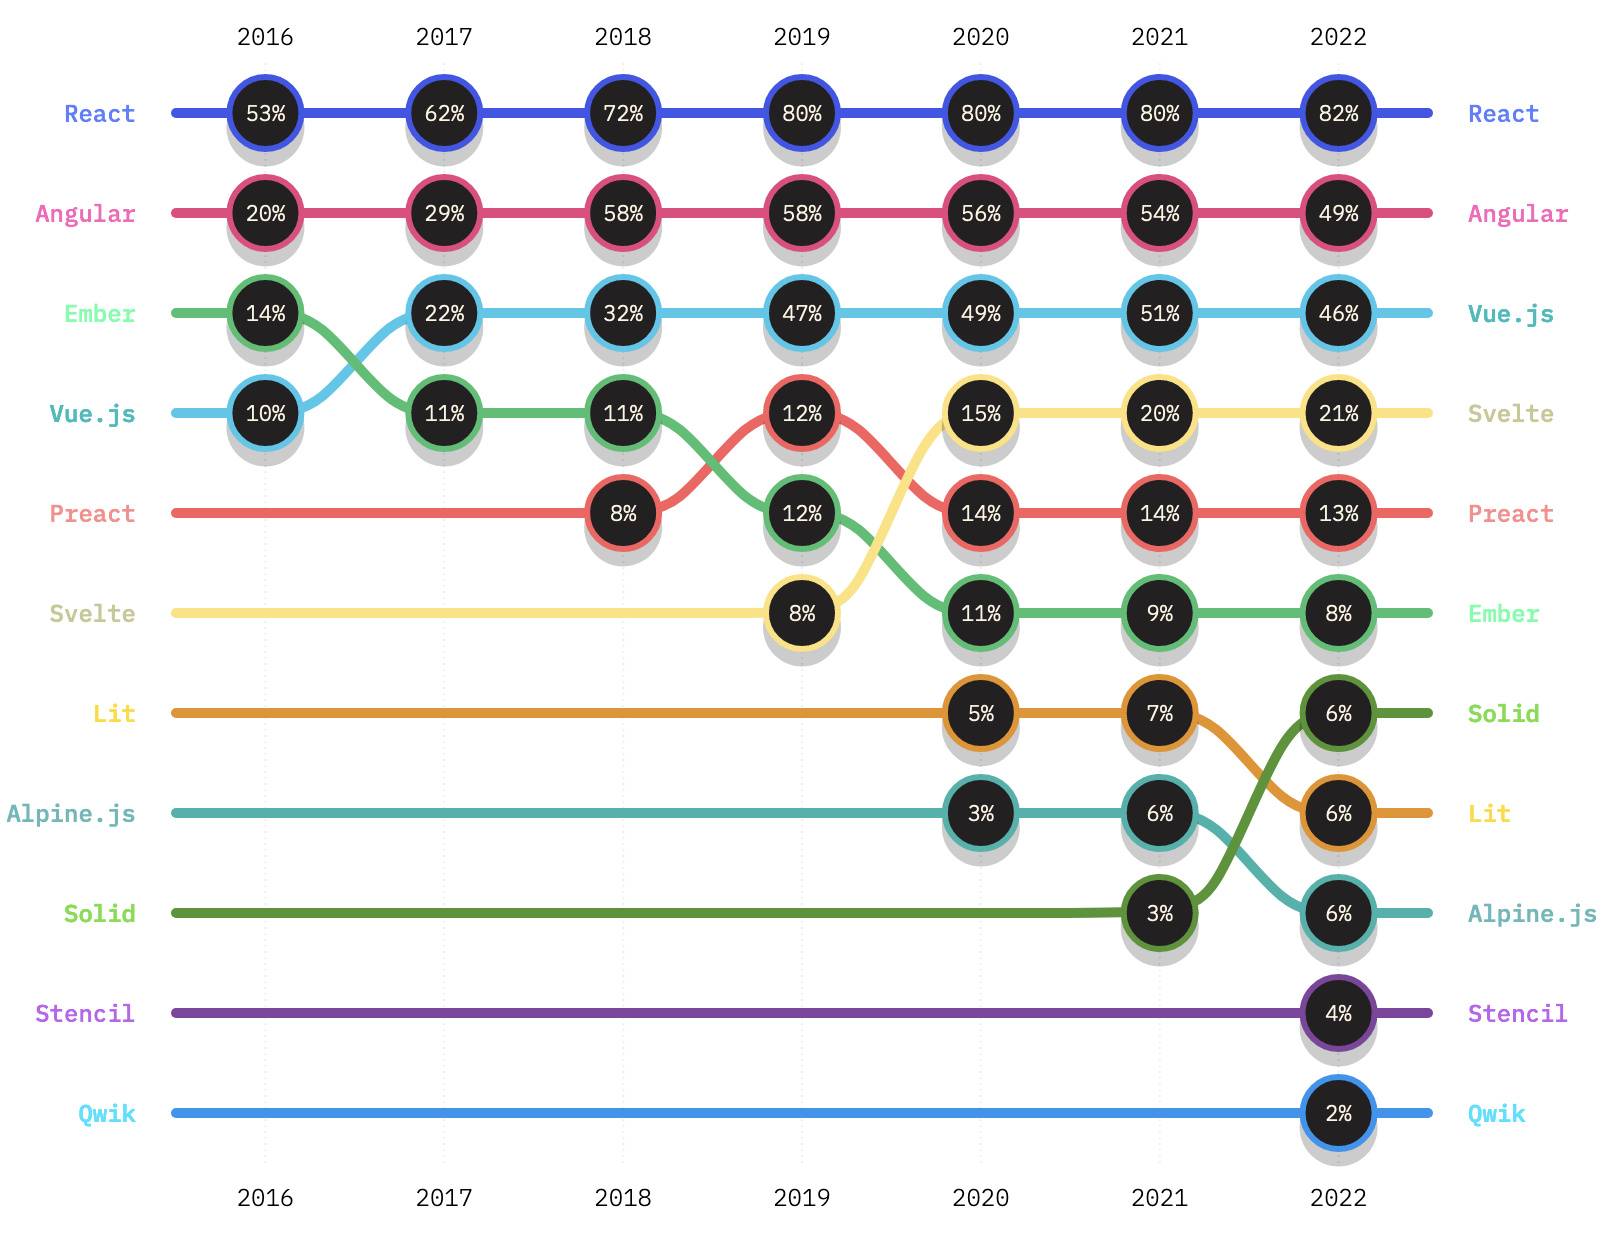
\includegraphics[scale=0.5]{04_Artefakte/01_Abbildungen/stateofjs-usage-frontend-frameworks-2022}
    \caption[Most used frontend frameworks in 2022]{State of JS: Most used frontend frameworks in 2022 \parencite{mostUsedFrontendFrameworks22}\protect}
    \label{fig:mostUsedFrameworks}
\end{figure}

\emph{React}\footnote{\url{https://react.dev}}, developed by Facebook in 2011 and maintained by its successor Meta, has become the most widely used tool for building \acp{SPA}.
It is steadily leading the rankings for most used frontend frameworks both in the Stack Overflow~\parencite{stackOverflowPollWebFrameworks23} and the State Of JS~\parencite{mostUsedFrontendFrameworks22} polls.
By definition, it is not a framework but a \ac{UI} library that relies on other extensions to support state management, routing and deployment functionality.
Although it is not a framework itself, there are existing frameworks like Next.js\footnote{\url{https://nextjs.org/}} for the web and ReactNative\footnote{\url{https://reactnative.dev/}} for building mobile apps using native functionality.
React makes use of \ac{JSX}, which allows directly mixing inline \ac{HTML} with the \ac{JS} or \ac{TS} source code.

\emph{Vue}\footnote{\url{https://vuejs.org/}} was developed by Evan You in 2013 and is maintained by an international team of individuals.
It had a relatively marginal presence in the US and Europe in the first years after its inception.
This can be partially attributed to its origin in China, as most of its supporting modules were localised in Chinese.
Over the years, it grew in popularity and received more international support, eventually overcoming the language barrier.
Unlike React, it is billed as a \textquote{progressive framework} that provides fundamental functionality for building reactive components but also accommodates more complex use-cases~\parencite{vueProgressiveFramework}.
Vue builds on standard \ac{JS} or \ac{TS}, \ac{HTML} and \ac{CSS} to create components, recommending a simple template mechanism mixed with reactive substitutions.
However, it also supports using \ac{JSX} for specifying inline \ac{HTML} within \ac{JS}.
As with React, there are extensions and frameworks like Quasar\footnote{\url{https://quasar.dev}} and Nuxt\footnote{\url{https://nuxt.com}} that enable more sophisticated workflows for application development and deployment.

\emph{Angular}\footnote{\url{https://angular.io/}} was initially released by Google in 2010 as AngularJS and officially discontinued in 2022.
A completely overhauled version 2 was released in 2016 and has since been maintained by Google.
It differs from React and Vue in that it is a complete framework containing everything required to build and deploy an application, and it explicitly recommends \ac{TS} as a programming language.
The framework is also less flexible because it is more opinionated and has its own set of best practices baked into the framework\textquotesingle s structure.

\section{Backend frameworks}
\label{sec:backend-frameworks}

The \emph{Express}\footnote{\url{https://expressjs.com}} framework provides the basic functionality to create web servers, including routing and middleware functionality.
TJ Holowaychuk developed it in 2010 and sold it to StrongLoop~\parencite{expressJsStrongLoop}, which IBM subsequently acquired~\parencite{expressJsStrongLoopIbm}.
It is currently under the stewardship of the OpenJS Foundation~\parencite{expressJsNodeFoundation}.
Express has become the de facto standard for building web services in JS, leading the ranking in the State of JS survey~\parencite{mostUsedBackendFrameworks22}.
Although it contains the necessary parts to create a web service, it does not enforce a specific architecture.
For developers who prefer a more explicitly defined structure, various other frameworks that add more opinionated structures or extensions are built on top of it.

Billed as a successor to Express, \emph{Koa}\footnote{\url{https://koajs.com}} is developed by the team behind Express.
It aims to provide a more robust and minimalistic iteration of the middleware-based architecture of Express.
Like Express, it allows for building a service from scratch in free form but is also the basis for other, more explicitly structured frameworks.

Other frameworks and a more stringent and structured application structure might be more desirable for complex applications.
Numerous \ac{JS} frameworks, some based on Express or Koa, and others that provide their own basis for routing.
To review all possible options is beyond the scope of this study.
In the following, three frameworks are selected for their specific nature related to popularity and stability, with an explicit focus on real-time applications.

\begin{table}[ht]
\centering
\caption{Backend frameworks ranked~\parencite{mostUsedBackendFrameworks22}\protect}
\label{tab:backendFrameworksRanking}
\begin{tabular}[t]{|l|r|r|}
\toprule
Framework & \% of question respondents & Stars on GitHub (k)\\
\midrule
\cite{githubNest} & 30.2 & 62.7\\
\cite{githubFeathers} & 8.8 & 14.9\\
\cite{githubMeteor} & 2.7 & 44\\
\bottomrule
\end{tabular}
\end{table}


\emph{Nest}\footnote{\url{https://nestjs.com}} is a backend framework for developers looking for a more strictly opinionated and robust setup than Express, e.g.\ for enterprise applications.
It follows a modular concept, making dependencies available to the services via injection.
Multiple database options exist, and transports can be both \ac{HTTP} and WebSockets.
There are \ac{CLI} scripts that enable automatic generation of boilerplate application code, and the language used to build Nest applications is TypeScript.
It ranks second among the most-used backend frameworks in the State of JS survey~\parencite{mostUsedBackendFrameworks22}.

The \emph{Feathers}\footnote{\url{https://feathersjs.com}} framework takes a different approach, making few assumptions about the specific application structure.
It uses aspect-oriented programming, a service-centric architecture and before-, after- and around-hooks (so-called \textquote{cross-cutting concerns}) for the services that modify basic behaviour or add functionality.
There are adapters for a wide range of databases and authentication methods.
The framework has a dedicated concept of channels that enable real-time functionality and messaging to clients.
Real-time transports are abstracted and can be deployed using Socket.IO or standards-compliant µWebSockets (see \autoref{sec:webstandards}). It also provides a \ac{CLI} to generate application code in \ac{JS} or \ac{TS}.
Feathers started as a hobby project by David Luecke and Eric Kryski in 2013~\parencite{feathersFrameworkHistory} and is currently maintained by David Luecke and a community of individual contributors.
It still ranks in the lower percentages in the State of JS survey~\parencite{mostUsedBackendFrameworks22}, but almost doubled that percentage from the previous one in 2021~\parencite{mostUsedBackendFrameworks21}.

\emph{Meteor}\footnote{\url{https://www.meteor.com}} explicitly focuses on real-time applications using WebSockets.
The framework is an outlier because while its core is open-source, other parts are proprietary code.
Nonetheless, it should be mentioned because it has been around for over ten years and uses WebSockets exclusively.
It was released in 2012 by a startup company, immediately received venture capital funding from Andreessen Horowitz and was eventually sold to Tiny Capital in 2019~\parencite{meteorSaleTinyCapital}.
The framework primarily uses MongoDB as a database system and initially provided its own package manager and ecosystem, build system, and template system based on Mustache\footnote{\url{https://mustache.github.io/}}.
Meanwhile, this exclusive strategy has been abandoned in favour of adopting the \ac{NPM}.
Still, it seems to be subject to debate regarding its ease of use versus its \textquote{growing pains} and related trouble with wide adoption~\parencite{meteorDiscussionYCombinator}.

\section{Databases}
\label{sec:databases}

\begin{table}[ht]
\centering
\caption{Multi-user databases ranking~\parencite{stackOverflowPollDatabases23}}
\label{tab:stackOverflowDatabasesRanking}
\begin{tabular}[t]{|l|r|r|}
\toprule
Database & \% of all question respondents & Stars on GitHub (k)\\
\midrule
\cite{githubPostgreSql} & 45.55 & 14\\
\cite{githubMySql} & 41.09 & 9.9\\
\cite{githubMongoDb} & 25.52 & 25\\
\bottomrule
\end{tabular}
\end{table}

\emph{PostgreSQL}\footnote{\url{https://www.postgresql.org}} is a very widely used database which uses a table-based data topology and implements \ac{SQL} for interaction with the database and its contents.
The relatively rigid database schema provides a solid structure for data storage and retrieval but, on the other hand, requires migrations to be written to transition from one database structure version to another.
It has an extensive feature set supporting complex data structures, \ac{GIS} data and data structured in \ac{JSON} format.
Developed in the 1980s at the University of California and switched to the \ac{SQL} in the 90s, it has remained a popular choice for enterprise and small-scale use.

Similar to PostgreSQL in that it also uses \ac{SQL}, \emph{MySQL}\footnote{\url{https://www.mysql.com}} supports many of the features of PostgreSQL, but has an overall smaller feature set.
It was initially developed in the 1990s by the private Swedish company MySQL AB and was forked as a completely open-source version in 2009 and renamed MariaDB\footnote{\url{https://mariadb.org}}.
It is still a popular choice, especially for smaller web projects that don\textquotesingle t need the extra functionality and value its relatively simple setup.

\emph{MongoDB}\footnote{\url{https://www.mongodb.com}} is a document store database that is designed to hold large amounts of unstructured data.
It has its own query language and features aggregation functionality that allows map/reduce and transformation operations or resolving of relations on the data before being sent to the client.
Although it uses the \ac{NoSQL} paradigm and allows storing documents of any kind in a collection, it eventually added the option of using schemas for validation.
It was initially released as open-source in 2009, then put under a proprietary license in 2018, but remains available for free usage with limited support~\parencite{mongodbProprietaryLicense}.

\section{Application deployment}
\label{sec:application-deployment}

\emph{Containerisation}, in the context of computing infrastructure, refers to the~\textquote[\cite{containerisationDefinition}]{packaging of software code with just the operating system (OS) libraries and dependencies required to run the code to create a single lightweight executable—called a container—that runs consistently on any infrastructure}.
It was popularised through the release of the Docker Engine\footnote{\url{https://www.docker.com}}, an open-source project devoted to creating an industry standard for application containerisation~\parencite{dockerRelease}.
The Docker team eventually launched the \ac{OCI} in 2015, which serves as~\textquote[\cite{openContainerInitiative}]{a lightweight, open governance structure (project), formed under the auspices of the Linux Foundation, for the express purpose of creating open industry standards around container formats and runtimes}.
It subsequently received Docker's container runtime as a donation, which was released as runC version 1.0 in 2020~\parencite{openContainerInitiative}.
It has recently become the de facto standard for packaging and delivering applications in web development and beyond.
GitHub reports that~\textquote[\cite{stateOfTheOctoverse23}]{in 2023, 4.3 million public and private repositories used Dockerfiles --- and more than 1 million public repositories used Dockerfiles for creating containers}.

\emph{Container orchestration} builds on the concept of containerisation. \textquote[\cite{orchestrationDefinition}]{Container orchestration automates the provisioning, deployment, networking, scaling, availability, and lifecycle management of containers.} The concept first gained popularity as Docker \textquote{swarm mode}, a functionality of the Docker software.
Still, its most successful instance so far is the software package Kubernetes\footnote{\url{https://kubernetes.io}}, which originated at Google in late 2013~\parencite{kubernetesHistory} and went on to be included in the \ac{CNCF}, a project by the Linux Foundation, that~\textquote[\cite{cloudNativeComputingFoundation}]{aims to advance the state-of-the-art for building cloud-native applications and services}.
It can be extended, highly customised and deployed on anything from an embedded device to a large-scale cloud infrastructure, providing a versatile deployment and management tool for many application infrastructures.

\chapter{Research methodology}
\label{ch:methodology}

This feasibility study was based on two essential parts.
The first was a reference implementation, providing insights into the work necessary for a basic functional implementation.
Based on this implementation, the application\textquotesingle s abstract performance was measured, an evaluation of the time spent on development was made, a qualitative review of the resulting codebase, and a critical reflection on the work process.

\section{Reference implementation}
\label{sec:reference-implementation}

To produce a valid test subject for the proposal, the reference implementation was created according to a prior selection of tools and methods deemed appropriate for the project.
The choices were made from the concepts and tools presented in \autoref{ch:conceptualfoundations}.

First, possible candidates were identified through internet research, and then at least three candidates were selected using the number of \textquote{Stars} received on GitHub as an indicator of popularity.
In some cases, other data sources had to be used where the technology predates GitHub (e.g.\ databases or programming languages), and its popularity should be judged by other means.
Developer surveys are being conducted by the popular technology forum Stack Overflow with over 90.000 participants for 2023~\parencite{stackOverflowPoll} and the \textquote{State Of JS} survey with over 20.000 participants that is more focused on web development~\parencite{stateOfJSSurvey}.
Additionally, GitHub publishes a yearly statistic on its public repositories, which helps identify technological trends and popularity among millions of open-source repositories~\parencite{stateOfTheOctoverse23}.
These sources provided additional input on popularity among a specific professional field and a general overview of technologies actively used.
The decision on choosing a candidate was made not by popularity alone, but with a stronger weight on a good fit to the project\textquotesingle s specific requirements and needs.
If a less popular framework did fit the specific development style, it would still be preferred to the popular status quo.
Another case might be a more recent project that has yet to collect as high of a rating on GitHub but presents a promising new approach or feature set.

The application development worked from the most basic boilerplate code towards finding the appropriate structure for the specific use case.
Well-known and easily defined components were built first.
The particular functionality of the reference implementation was then built on top in constant cycles of adding functionality, reviewing the codebase and refactoring towards abstraction and separation of basics from specifics.
As only a rough architectural model for the project was defined beforehand, tests and documentation were written later in the process, as the parts stabilised independently and in their relationship with each other.
This method does not strictly adhere to standard development procedures.
Still, it borrows loosely from agile development (sprints, reviews, adjustments) and simple forms of the ideas put forward in the book \textquote{Pattern-Oriented Software Architecture}, such as application partitioning through layering, separation, and standardised messaging~\parencite{patternOrientedSoftwareArchitecture}.
A more systemic approach for the development process, like application modelling using \ac{UML} and test-driven development, might be desirable for teams, but the various and disparate \textquote{moving parts} in conjunction with heavy reliance on browser-only \ac{API}s complicate the creation of a well-simulated testing environment using either real or mock-data, especially for a single developer.

The application was implemented in its entirety, documented, packaged and deployed.
Appropriate test coverage was provided for the core functionality, and the overall time spent was logged in timesheets and categorised by the general work areas.
The application\textquotesingle s server components were deployed early on to university hardware and made available over the internet.
The client application was then run and tested on exemplary computer systems in and outside the university network.

\section{Analysis and evaluation}
\label{sec:analysis-evaluation}

A statistical analysis of the timesheets provided insight into the \emph{workload} time spent on various aspects of the software.
It differentiated between languages and application components to provide insights into the feasibility of setting up such a system from scratch with a single developer and the potential cost of just reworking the parts deemed transient and related to the specific use case.

The application\textquotesingle s \emph{performance} was tested regarding the load put on the \ac{CPU} (server and client) and the network throughput and latency.
It was verified that all message processing worked as expected through unit testing and simple manual testing tasks performed on the application.
A practical test that analyses the actual user experience and uses performers and real dance interaction was deemed beyond the scope of this study.

The \emph{code quality} was assessed based on volume (source code files and lines of code without comments) and cognitive complexity, ~\parencite[see][]{sonarSourceCognitiveComplexity}, which is an updated version of the older concept of cyclomatic complexity, which counts the number of linearly independent paths throughout a piece of code~\parencite[see][]{mcCabeComplexity}.
It was published by the Swiss company SonarSource\footnote{\url{https://www.sonarsource.com/}} and \textquote{has been formulated to address modern language structures, and to produce values that are meaningful at the class and application levels}~\parencite[4]{sonarSourceCognitiveComplexity}.
It accounts for modern control structures and aims to facilitate legibility by rewarding a code style that benefits general understandability~\parencite[4]{sonarSourceCognitiveComplexity}.
Both metrics should be kept low for each source code file, as code with many lines makes it harder to read, and high complexity is more challenging to follow and understand.
The code volume is difficult to reduce to a static maximum, but \textquote{the [\ac{SATC}] has found the most effective evaluation is a combination of size and complexity}~\parencite[6]{softwareMetricsReliability}, so a self-imposed threshold should be set, even if exceptions are made later.
For \ac{OOP}, limiting a file to a single class is often advised.
Still, depending on the language used, the file can also contain multiple functions that are better grouped instead of scattered across various files.
A general rule of thumb proven to be a good measurement from experience is that a single file should be at most 160 to 200 lines of code (without comments) to skim it and get a general overview quickly.
There are exceptions to these rules where a specific function or class exceeds this threshold, but breaking it up would not make it easier to understand.
In those cases, there can be a discussion about changing the general application design to partition the functionality differently.
Alternatively, it can be decided to keep this code and improve documentation.
Reducing volume and complexity is especially important if the code should be passed on to others who want to maintain and modify it for further use.
Here, the general idea was that the transient (hackable) parts (e.g. \ac{UI}) should be kept as simple as possible, avoiding unnecessary complexity.
The more static and stable core components would then be where the complex code would be moved to (e.g.\ the core \ac{SDK}).

Additionally, a \emph{critical reflection} and analysis of the development process was created to weigh the expectations against the experiences while implementing the decisions made in planning the application.
It evaluated general reproducibility and feasibility and discussed the benefits and limitations of establishing a task-specific application from scratch using the proposed concept.

\chapter{Application concept}
\label{ch:concept}

The reference implementation was named \emph{Sensorama}, a reference to the early immersive experience patented by filmmaker Morton Heilig in 1962~\parencite{Heilig_1962}.
It is said to be the first virtual reality system~\parencite[5][]{vrHistoryGigante} and features stereoscopic video and audio, simulated wind and even olfactory stimuli.
The name is a nod to the longstanding history of ideas around immersive experiences mediated through machinic technology and the multisensory approach that, in this case, refers to the many possible input and output methods.
Although the reference implementation was not designed to support an actual artistic process, its development was informed by past practical experience working with technology in performance, specifically in a dance context.
While the application\textquotesingle s base functionality could theoretically be used for any number of participants, only limited by the infrastructure\textquotesingle s resources, it was specifically designed for only two active participants at a time.
This decision was made because it would already be a challenge to adapt to relating to a mediated presence only by localising it acoustically and at the same time focusing on sound cues to base one\textquotesingle s own movement on.
However, a passive option of viewing the virtual space was included, allowing the use of \ac{WebXR} functionality to join as a spectator.

\section{Architecture}
\label{sec:architecture}

Due to the containerised packaging and deployment, the application can be deployed in any cloud environment or other hosting platform providing virtual or dedicated hosts with root access.
The underlying software infrastructure requirement is minimal, and the required components are a Linux \ac{OS} with installations of Docker (with ContainerD) and Kubernetes.
No special hardware is needed, and the system can run in any environment that provides network access, storage space and standard computing resources.
The underlying general architecture was partitioned into three essential parts (\autoref{fig:sensoramaStack}).
The general infrastructure is thought of as any kind of Kubernetes installation, either on \textquote{bare metal} or a virtual server instance.
Running on top of that is a set of base applications (\ac{API} and \ac{WebRTC} server), which would ideally be the same across multiple deployments of the actual implementation.
The \ac{UI}, which holds the use-case-specific functionality, could then be forked, modified and duplicated multiple times using the same basic architecture.

\begin{figure}[!ht]
\centering
\includesvg[scale=0.8]{04_Artefakte/01_Abbildungen/sensorama-stack}
\caption[Sensorama stack diagram]{Partitioning the Sensorama technology stack\protect}
\label{fig:sensoramaStack}
\end{figure}

While all the frameworks presented in \autoref{fig:mostUsedFrameworks} could be used to build an application as envisioned in this study, Vue was selected due to the relatively high acceptance and the comparably easy learning curve.
While it might not be the choice for large-scale or enterprise apps, the low entry barrier and the simple structure make it ideal to get an app up and running quickly, experiment with it and pass it on to others for hacking and custom modifications.
The Quasar framework was used to accelerate and simplify the initial development (see \autoref{sec:frontend-frameworks}).
It extends Vue\textquotesingle s basic functionality with a \ac{UI} library complete with layout tools, common interface elements and a comfortable development and deployment environment.

The choice for a backend framework landed on Feathers and, by extension, Koa.
The simple structure and code generators allow for a speedy setup and deployment of a simple WebSockets \ac{API} that provides authentication and resource management.
It was connected to a MongoDB database because there was no definitive initial plan for how the stored and retrieved resources would be structured and typed.
Using a flexible document store, the data could be easily overwritten with updates and then wiped before the schema would eventually be deemed stable.

LiveKit was chosen as the WebRTC server implementation because it is versatile, and there is an easy installation method to set it up as a container running alongside the Redis database in Kubernetes.
While Mediasoup might have allowed a more precise implementation and probably a more efficient one, the workload overhead for building everything already offered by LiveKit was deemed too much effort for this kind of application.

\section{Design paradigms}
\label{sec:design-paradigms}

The basic design paradigm chosen for the Sensorama application was that of an \ac{SPA}.
As a remote API was already involved in managing access to shared resources, the extended \ac{PWA} paradigm was not helpful for this scenario.
It was designed as an exclusively real-time application that uses WebSockets for all transmission between app components and uses the WebRTC standard for user communication.
The project was structured as a monorepo, where all components were developed across different languages in a single repository.

The application\textquotesingle s custom part was partitioned into the \ac{UI}, which was deployed as a statically compiled \ac{HTML}/\ac{CSS}/\ac{JS} bundle, the \ac{API}, which was set up as a single-process Node.js application and the so-called \textquote{Data-Producers}, which are external native utilities written in Python and C++ that provide bridges to motion capture hardware.

The primarily favoured coding paradigm was \ac{OOP}, but this was not strictly enforced for all components.
As some frameworks prefer different, more functional paradigms that are also compositional (Vue) or aspect-oriented (Feathers), it was deemed appropriate to refrain from enforcing a singular coding style.
While this might usually be considered bad practice in terms of maintainability for long-term development, it served the purpose of a modular and somewhat transient \textquote{single-use} application structure.

An essential part of the development concept was the sequence of development phases.
As there was no explicit definition beforehand, the development started by establishing a functional skeleton first and worked within that to carve out the actual functionality.
Initially, monolithic large blocks of code were written with little initial planning.
Various approaches to desired functionality were quickly tried and discarded or kept and subsequently extracted into separate components grouped by functional association.
Using this strategy, it was essential to review and refactor regularly and often to allow the application structure to emerge from what otherwise would dissolve into the colloquially termed \textquote{spaghetti code} and to avoid unnecessary side-effects among the components.
The core features were extracted into a separate \ac{SDK} module towards the end of the development process, and appropriate unit tests were written.
The application could now move into practical testing, similar to a production deployment, and thus, the core functionality needed to become more rigid and covered by test cases.

The general \ac{UI} and data producers were considered transient because they served only the singular use case and should be subject to frequent future modifications.
These application components should be hackable and replaceable, so they were not formally tested, at least in the scope of this study.
The unit testing focused on the data input and output for the core functionality to provide a stable foundation by keeping all components connected in a unified messaging system.
By modelling the basic request and response cases and formulating them as tests, potential later users would also have a tangible way of understanding the application\textquotesingle s core mechanics.

For \ac{JS}, three popular testing frameworks are Jest, Mocha, and Jasmine (\ref{tab:githubTestingFrameworks}), which can be used for implementing unit testing for the project.
In this case, the selection skipped the most popular option of Jest in favour of Mocha, which is used by the Feathers \ac{API} framework in its generator for boilerplate code.
This way, basic tests to base work on were already available and, to keep the project consistent across modules, were adopted for the core \ac{SDK} module.

\input{04_Artefakte/02_Tabellen/github_testing_frameworks_stars}

\section{Movement quality extraction}
\label{sec:movement-quality-extraction}

One quality chosen was the \textquote{average velocity}, generally defined as the distance travelled over time (e.g.\ m/s).
Additionally, two more specialised concepts, developed for expressive movement analysis, were selected: \textquote{Quantity of Movement}~\parencite[96-97]{movementQualities}, describing the amount of difference between poses over time, and the \textquote{Contraction Index}~\parencite[97]{movementQualities} which observes the density of space used by a pose.

While the former is easily defined as the velocity calculated for a singular point (the centre of mass with an equal distribution), the latter two have been initially developed to observe pixelated \ac{2D} camera images and needed to be translated to \ac{3D} space.
To transfer the methods to \ac{3D} space, Open3D\textquotesingle s PointCloud class was used~\parencite{open3DPointCloudReference}.
In the case of the \emph{quantity of movement}, the original proposed method of difference detection is based on the percentage of changed pixels in a \ac{2D} silhouette.
This concept was transferred to \ac{3D} by now comparing the points that make up the point cloud or pose provided by the capture hardware by using the function for computing point cloud distance, that \textquote{for each point in the source point cloud, compute[s] the distance to the target point cloud}~\parencite{open3DPointCloudReference}.
This list of distances was then filtered by the entries exceeding a threshold (e.g.\ 0.01~metres), providing the basis to calculate a percentage of changed points (see \autoref{listing:quantityOfMovement3D}).

\begin{listing}[!ht]
\inputminted{python}{04_Artefakte/03_Listings/quantity-of-movement.py}
\caption{Using Open3D for calculating the quantity of movement in \ac{3D}\protect}
\label{listing:quantityOfMovement3D}
\end{listing}

The original \emph{contraction index} is based on the ratio of space within a bounding box covered by the pixels of the silhouette enclosed by the bounding box.
This was translated to \ac{3D} by using an axis-aligned bounding box and a convex hull instead of a silhouette and then taking the ratio of bounding box volume to convex hull volume to get the percentage of space \textquote{covered}, which is the contraction index (see \autoref{listing:contractionIndex3D}).

\begin{listing}[!ht]
\inputminted{python}{04_Artefakte/03_Listings/contraction-index.py}
\caption{Using Open3D for calculating the contraction index in \ac{3D}\protect}
\label{listing:contractionIndex3D}
\end{listing}

All three qualities were smoothed using a moving average of five frames to reduce jitter in the values.

\section{Sonification method and sound spatialisation}
\label{sec:sonification-method-and-sound-spatialisation}

The three basic movement qualities extracted provided the basis for a reference pipeline implementing parameter mapping sonification (see \autoref{sec:movement-data-sonification}).
The movement qualities were made available to the application, enabling an event-based system where thresholds that switch a boolean value at the crossing time can be defined.
As these values are watched, events can be triggered depending on their on- or off-state.
At the time of an event, the current value of a quality or a combination of them can be used to determine the magnitude of the event\textquotesingle s impact.

A simple system of scales, chords, and note selection was introduced to create an example sonification algorithm.
The system was based on selecting a specific scale (e.g.\ E-minor) for which a list of possible chords could then be produced.
Each time an event is triggered on one of the qualities (e.g.\ quantity of movement), the actual value can be used to decide which chord to select from the list using the normalised value.
The notes selected from the chord are then transposed using another quality (e.g.\ contraction index), selecting the root note for the chord across the octaves.
The average velocity was used to set the note length, triggering shorter notes when standing relatively still and more extended notes while travelling in space.
It must be noted that while this is a valid example for a parameter mapping sonification and will produce largely harmonic notes, it falls short of producing an output of a more complex musical quality because it lacks the ability to construct deeper structures and dramaturgic variance.
However, if engaged over a more extended period and practised, it could still yield interesting results, but this would also require a very specific way of composing the movement required to produce musically exciting results.

All handling of harmonic structures such as scales, chords and notes is done using the \ac{JS} library Tonal\footnote{\url{https://tonaljs.github.io/tonal/docs/}}, which provides a comprehensive library for working with western musical theory.
The audio framework chosen was Tone.js, as it was the most straightforward option focusing on musical applications.
It allows selecting an audio file added as a static asset in the \ac{UI} set to a specific root note that is then triggered in the correct pitch for the note selected with variable attack and sustain times.
While Elementary seems very promising in its approach to sound generation, it is much more low-level in its approach to constructing an instrument for music generation.

Sound spatialisation was achieved by playing the notes through a spatial sound source node placed within a virtual audio scene configured with reflecting floor, walls and ceiling, provided by the Resonance audio framework and based on the WebAudio \ac{API} (see \autoref{subsec:webaudio}).
The audio stream retrieved from the \ac{WebRTC} connection and the sound produced from the synthesiser nodes for the local and remote participants were connected to their respective spatial panner nodes.
If the participant's head orientation and position were available through motion capture or the head tracking device, this spatial information would also be applied to the listener node and the other spatial audio nodes.

\section{Messaging}
\label{sec:messaging}

Standards-compliant protocols enabled streamlined messaging among the disparate application components based on different languages and run in various environments (see \autoref{fig:messagingFlow}).
Starting on the client side, the motion capture data producer starts a local WebSockets server to which the web application running in the browser can connect and receive live data.
The browser application can connect to the custom head-tracking device using the WebBluetooth standard and receive data messages using the \ac{GATT}\footnote{\url{https://www.bluetooth.com/bluetooth-resources/intro-to-bluetooth-gap-gatt/}}.

The conferencing functionality implemented in the web application was used to send local microphone audio and to relay the local producer utilities\textquotesingle\ data to other participants via the LiveKit server using the WebRTC protocol.
In the backend, the LiveKit server can push status updates as \ac{HTTP} webhook calls to the \ac{API} server to notify it about connects and disconnects.
The \ac{API} server uses the WebSockets protocol to relay updates on persisted data and LiveKit update events to the client browser and receives authentication and general data requests.

\begin{figure}[!ht]
\centering
\includesvg[scale=1.0]{04_Artefakte/01_Abbildungen/application-messaging-flow}
\caption[Application messaging flow]{Messaging flow between the application's components\protect}
\label{fig:messagingFlow}
\end{figure}

\section{Data modeling}
\label{sec:datamodeling}

Four core data models were defined for the application (see \autoref{fig:apiDataModel}).
The two models persisted by the \ac{API} server are \emph{Spaces} and \emph{Users}.
These were modelled as simple reference objects providing the basis for connecting users to virtual spaces, akin to spatial chat rooms, and each User can own multiple Space objects.
A Space is a container object representing a shared space populated with multiple participants\textquotesingle\ sensor readings.
Users can request one or more \emph{Token} objects that allow them to connect to a \textquote{room} on the LiveKit server that maps to a specific ID of a Space.
Once connected, the LiveKit server notifies the \ac{API} server of the new connection, and now the connected participant\textquotesingle s ID can be found in the list retrieved from the virtual \textquote{connected} property of the Space object.

\begin{figure}[!ht]
\centering
\includesvg[scale=1.0]{04_Artefakte/01_Abbildungen/api-datamodel}
\caption[API data model]{Basic data model used in API server\protect}
\label{fig:apiDataModel}
\end{figure}

The connected participants can exchange arbitrary \emph{data messages}.
The data messages were not designed to be encoded as \ac{JSON} text messages but sent as raw data to make them as small as possible.
Messages were structured as byte sequences, with a 64bit long integer timestamp using the first eight bytes, then a single byte with an unsigned integer for selecting a message schema from the enumerated message types and a freely defined sequence of different number types (\autoref{fig:messageStructure}).
32-bit floating point numbers were used for all sensor readings as the numbers stay sufficiently small, and the precision is enough for millimetre measurements, statistical values or angles.
The numeric values were encoded in \ac{LE} format~\parencite{cohenEndianess} that appeared consistent across all environments but should be explicitly adhered to if other components were to be added to the application.

\begin{figure}[!ht]
\centering
\includesvg[width=\textwidth]{04_Artefakte/01_Abbildungen/generic-message-structure}
\caption[Generic Message Structure]{The basic message structure for transmitting numeric sensor readings\protect}
\label{fig:messageStructure}
\end{figure}

The message schemata were described in \ac{JSON} files to make them available across languages.
Shown in \autoref{listing:exampleMessage} is a simple example message schema for a nanosecond timestamp (\emph{{t\_ns}}), \emph{type} and one or more \ac{3D} \emph{points} stored as floats.

The root object\textquotesingle s property names resolve to the key under which the value could later be accessed.
The \emph{index} property specifies the byte index in the message, and \emph{count} specifies if the value repeats in sequence or is singular. \emph{dims} defines the dimensions for the value (e.g. \textquote{3} for a \ac{3D} point).
The \emph{type} could be a \textquote{Uint8}, \textquote{Float32} or a \textquote{BigInt64} and the boolean property \emph{le} specifies if this value is encoded as \ac{LE}.

\begin{listing}[!ht]
\inputminted{json}{04_Artefakte/03_Listings/example-pose-message.json}
\caption{Example pose message schema}
\label{listing:exampleMessage}
\end{listing}

\section{Application components}
\label{sec:application-components}

The application comprises several third-party components merely deployed as-is (WebRTC, databases, static web server) and the custom-developed parts described in the following section.

\subsection{Core SDK module}
\label{subsec:core-sdk-module}

The core functionality was built into a separate module to enable integration into other setups using different frameworks or architectures.
The module uses the \ac{NPM} package format and can be utilised in the browser and Node.js.
While this module carries the most fundamental functionality, it was created last in the development process, as the essential parts only crystallised during the initial development phase.

\subsection{User interface}
\label{subsec:user-interface}

The user \ac{UI} provides the main entry point for the users.
It allows authentication via a local username and password combination.
It provides objects modelled as virtual \textquote{spaces} that are the central anchor to organise all communications, as defined in \autoref{fig:apiDataModel}.
Users can create spaces, name them and then join them, becoming active data producers, or choose to view them as passive spectators.

Depending on the participant\textquotesingle s role, a space is rendered as a different set of components.
Participants who actively join have access to a local data producer and a head tracker control panel.
These components provide a direct link via WebSockets to the external data producer utilities, and a WebBluetooth connection to the custom head tracking device built using an Arduino.
Those who only view the space do so via a dedicated scene viewer component that brings together all incoming streams and signals.

The \ac{UI} was designed to coordinate the connections between the WebRTC server, the backend \ac{API} and the local utilities.
It also implements the various web standard \acp{API} needed for sound, graphics and communication.

\subsection{API server}
\label{subsec:api-backend}

The \ac{API} server was tasked with managing the basic connecting objects (spaces and users), general authentication, and generation of access tokens for the LiveKit server.
Using its real-time channels, it can notify connected clients of changes like other connecting users or updates to data.
The Feathers framework exports its own client library that is specifically generated for the current server configuration.
It can be directly integrated into Vue using a client adapter module that handles authentication and basic \ac{CRUD} operations.

\subsection{Native utilities}
\label{subsec:native-utilities}

Three different native utilities were additionally implemented.

The general \emph{data producer} was set up as a \ac{CLI} utility in Python, implementing various Python-specific extensions: the DepthAI framework\footnote{\url{https://github.com/luxonis/depthai}}, used to work with the Luxonis Oak-D line of \ac{3D}-cameras, Intel\textquotesingle s OpenVino\footnote{\url{https://github.com/openvinotoolkit/openvino}} for interacting with various \ac{ML} models for pose recognition or point-cloud extraction, Open3D~\parencite{open3DZhou2018} for working with point cloud data and performing general spatial operations and PyMotion~\parencite{githubPyMotion}, a library for working with recorded \ac{BVH} motion capture data files.
Python also allowed for easy statistical data analysis using NumPy, which was used to perform movement quality extraction.

For real-time streaming of live motion capture data from the Captury Live system, there currently only exists a C++ client library provided by the system's manufacturer.
Thus, the \emph{Captury data producer} component had to be implemented separately and uses a C++-based WebSockets server streaming the library's received data.

As there was no affordable, open and platform-independent \emph{head-tracking} solution, this component was quickly prototyped using a BluetoothLE-ready Arduino device and an \ac{IMU} component for absolute orientation measurement by Adafruit that can be directly connected to the Arduino using the \ac{I2C} serial bus.
The data read from the \ac{IMU} device was then posted as binary messages on a simple Bluetooth service.
The device could be directly integrated using the browser\textquotesingle s WebBluetooth web standard.


\chapter{Implementation}
\label{ch:implementation}

\section{Project Setup}
\label{sec:project-setup}

The underlying \emph{server infrastructure} for the reference implementation was an existing server with 16 \ac{CPU}-cores (with multithreading), 64 \ac{GB} \ac{RAM} and a 512 \ac{GB} \ac{SSD} drive, located on the \ac{JGU} campus and connected to the internet via a dedicated one-gigabit network connection (see speedtest\footnote{\url{https://www.speedtest.net/}} results in \autoref{listing:speedtestServer}).

\begin{listing}[!ht]
\inputminted{text}{04_Artefakte/03_Listings/speedtest-server.txt}
\caption{Speedtest: connection statistics for the server used to deploy the application\protect}
\label{listing:speedtestServer}
\end{listing}

The orchestration was deployed first to allow development on a working remote WebRTC infrastructure.
The basis was a clean, freshly bootstrapped Kubernetes installation running on the bare-metal server.
LiveKit and its Redis database were installed via the application deployment manager Helm, using an official installation chart published by its maintainers\footnote{\url{https://github.com/livekit/livekit-helm}}.
To simplify the deployment, LiveKit was placed behind the reverse proxy Traefik\footnote{\url{https://traefik.io/}} to manage \ac{SSL} termination via the LetsEncrypt\footnote{\url{https://letsencrypt.org/}} service and routing to the actual service running inside the cluster.
However, this simplified setup required LiveKit to be configured to listen on a single \ac{TCP} port instead of a range of UDP ports, as it would usually be deployed.
The potential downside of this deployment configuration was deemed insignificant since the server only needs to service a handful of users.
The detailed Kubernetes setup instructions are documented in the according folder in the project\textquotesingle s repository\footnote{Kubernetes setup instructions: \href{https://github.com/dasantonym/sensorama/tree/master/kubernetes}{https://github.com/dasantonym/sensorama/tree/master/kubernetes}}.

The \emph{LiveKit} installation was deployed with only a slight deviation from the default configuration.
It was set up to use \ac{TCP} as a transport protocol to allow easier integration with \ac{SSL} termination using the reverse proxy.
Otherwise, the configuration defined the endpoints for sending webhook requests and custom credentials for making requests to it via the server-side \ac{SDK} and generating valid access tokens for users to connect to rooms.
The Helm installation chart was used to set up the system along with its Redis database installation in a single command, and the server was immediately ready for connections.

The development process was conducted in a desktop environment, using the suite of tools developed by JetBrains (WebStorm, PyCharm and CLion), as these are free for educational use and provide a complete environment for development, including debugging, intelligent code completion, versioning, containerisation and deployment.
A local Docker Desktop installation allowed running services and databases locally to support development before publishing to the production environment.
Versioning was done via Git on the GitLab platform provided by the \ac{JGU}\footnote{\url{https://gitlab.rlp.net}}.

\section{API server}
\label{sec:api-server}

The first custom implementation, the \ac{API} server, was generated using the Feathers \ac{CLI} tool with standard username and password authentication and WebSockets, as well as \ac{HTTP} transports, enabled.
It provides the core services for Users, Spaces, Tokens and LiveKit events.
These services were autogenerated using the Feathers \ac{CLI} utility.
They were used largely unmodified, except for adding the properties on the models for Users and Spaces as defined in \autoref{sec:datamodeling}.
A custom service class was added for the Tokens, as these do not persist in the database and instead are generated on the fly by the LiveKit server \ac{SDK}.
All other boilerplate code for the \ac{API}, including the MongoDB integration, the authentication mechanism, and the REST and WebSockets transport integrations, were also autogenerated using the \ac{CLI}.
An additional custom Livekit event service was added to the API, allowing it to receive webhook requests via \ac{HTTP} from the LiveKit server containing updates on connecting and disconnecting users.
These events do not persist in the database but are relayed instead to the connected users via the real-time channels.
The channels feature provided by Feathers was used to automatically subscribe, connecting users to updates on the services for Spaces and Livekit events.

\section{Core SDK}
\label{sec:core-sdk}

The basic functionality was bundled in an \ac{NPM} module to make the base code independent of the use case, which could later be used in other projects.
This module contains the abstract classes \textquote{DataProducer}, \textquote{HeadTracker} and \textquote{SonificationController} alongside the message specification for the various types of transmitted data.
It was written to propagate updates via events instead of the reactive patterns used in Vue so that it can also be used independently from the framework used for the study.
Unit tests were added to the module to maintain a stable implementation.

\section{User interface}
\label{sec:user-interface}

The Quasar framework provides a \ac{CLI} to generate new projects, which allows selecting basic implementation details (e.g.\ language, state management) and producing a complete and working empty Vue project with sample components that served as the starting point for the \ac{UI} implementation.
The first thing added to the project was the library \textquote{feathers-pinia}\footnote{\url{https://feathers-pinia.pages.dev}}, which is provided by the Feathers developer community and promises easy integration of an existing Feathers \ac{API} with any Vue project using the Pinia\footnote{\url{https://pinia.vuejs.org/}} state management system used by Vue.
The extension was integrated by linking the client library that the Feathers server project automatically generates by referencing the \ac{API}\textquotesingle s project folder and configuring basic authentication settings.
The routing configuration and page components were set up according to the sitemap (see !!!autoref{fig:sitemap}).

The overview page for the spaces presents a list of the names alongside the currently connected users and buttons to either join as a participant or passively view it as a spectator.
On joining a space, the user first needs to activate their microphone to activate the audio context.
The user is then presented with three basic control panels.
The \textquote{Data producer} panel allows setting a URL of a local WebSockets server published by a data producer, setting the message type received from it, and optionally enabling a tracing function to log the packet transmission statistics.
Once connected, the panel shows a preview of the incoming points data, transmission statistics and a button to disconnect.
Internally, the panel creates a reactive data store that instantiates the \textquote{DataProducer} class from the core \ac{SDK}, watches incoming message events and populates the received data as reactive properties to be used across the \ac{UI} in various other components without the need of creating additional class instances.
The second panel, \textquote{Head tracker}, works similarly but uses the Web Bluetooth \ac{API} to select a nearby device and connect to it to receive its data messages.
The third component configures the sonification by setting thresholds on incoming movement quality values.
It connects to an instance of the \textquote{SonificationController} class from the core \ac{SDK} and allows the configuration of event thresholds, sound selection and tonal configuration.

When using the page to view a space, there is only one component, the \textquote{SpaceViewer}, that shows a \ac{3D} room in which all incoming points are rendered as small spheres, giving the impression of a human figure.
For each participant, there is a differently coloured light source that follows the centre of mass of the points associated with the participant.
The viewer also renders all sonifications and audio streams at their respective spatial positions.
This allows the user to view the \ac{3D} scene on screen while listening to binaural audio or to use the built-in \ac{VR} functionality to experience the scene in a visually immersive way.

\section{Data producers}
\label{sec:data-producers}

The general \emph{data producer} was written in Python and provides multiple data sources: an interface to a Blazepose implementation on the Oak-D \ac{3D} camera, as well as reading depth images as point clouds from the camera and an interface to load and playback motion capture data in the \ac{BVH} file format.
All three data sources were implemented as separate Python classes because the classes related to the Oak-D camera were built by modifying existing code for pose recognition~\parencite{githubDepthAiBlazePose} and point cloud processing~\parencite{githubDepthAiPointcloud}.
The \ac{BVH} data source was created from scratch and implemented to facilitate testing and development by using playback of motion capture data of professional dancers pre-recorded on the Captury Live system.
All data source classes were set up to support calling a function in a loop and returning current point data as a multidimensional array.
The returned data is packed as a byte sequence and sent over WebSockets in the appropriate format (see \autoref{sec:datamodeling}).
This way, the disparate sources could be imported into a single central file that uses a combined set of utility functions for running a WebSockets server and packing data.
Due to the lack of a Python-based client for the Captury Live system, the Captury producer had to be implemented separately as a C++ project using CMake\footnote{\url{https://cmake.org/}} as a build system and based on the \textquote{RemoteCaptury} client library~\parencite{githubRemoteCaptury}, as well as an example project for a WebSockets server implementation in C++~\parencite{githubCppWebSocketsDemo}.

The custom-built head-tracking device was implemented as an Arduino project.
As such, it was first realised as a hardware setup and then outfitted with custom firmware written in the Arduino-specific flavour of C/C+.
The hardware implementation was created using the \textquote{Arduino Connect RP2040}\footnote{\url{https://docs.arduino.cc/hardware/nano-rp2040-connect/}}, which is based on the Raspberry PI 2040 microcontroller and has an onboard BluetoohLE module.
The \ac{IMU} module used was the \textquote{9-DOF Absolute Orientation IMU Fusion Breakout}\footnote{\url{https://www.adafruit.com/product/4646}} which uses the BNO055\footnote{\url{https://www.bosch-sensortec.com/products/smart-sensor-systems/bno055/}} chip produced by Bosch.
This chip has the benefit of already pre-processing the data from the gyroscope, accelerometer and magnetometer into an absolute world position that can be directly read from the breakout board via the \ac{I2C} bus.
As a third component, a small 3.7V lithium battery was added alongside a charging module\footnote{\url{https://www.adafruit.com/product/1905}}.
Only six connections needed to be soldered between the three modules (2x charger and 4x \ac{IMU}), and the resulting circuit was ready to function as a custom head tracker.
For the software implementation, the basic example code for the Adafruit module was used to set up continuous polling of the positioning module, reading the values for position and device calibration status and sending them as byte sequences at a fixed rate of ~25fps over BluetoothLE\@.

\chapter{Discussion}
\label{ch:discussion}


\section{Application performance}
\label{sec:statistics}

The statistical evaluation focused both on the extrinsic properties of the application and the development process itself (e.g.\ code volume, complexity, time spent on development), as well as the intrinsic functional properties of the core functionality that are reflected in the cost of \ac{CPU}-, network-usage and message latency.
The cost of rendering audio and video, as well as general user experience metrics, were beyond the scope of the study, as these are highly specific to the task being implemented and are considered transient.

Two computers used in the performance evaluation were end-user laptops with the following specifications:

\emph{Computer A} was equipped with a dual-core Intel Core i5 \ac{CPU}, 16~\ac{GB} of \ac{RAM} and a 500~\ac{GB} \ac{SSD}.
\emph{Computer B} was equipped with an Apple M1 Max \ac{CPU} with ten cores, 64~\ac{GB} of \ac{RAM} and a 1~\ac{TB}~\ac{SSD}.

The test systems were located in a rural area 80~\acp{km} outside Mainz, used the Google Chrome browser (version 121.0.6167.85), ran macOS~13.6.4 and connected to a consumer \ac{ADSL} connection (60~\ac{Mbit} download and 15~\ac{Mbit} upload) via an 802.11ac wireless connection (\autoref{listing:speedtestClient}).

\begin{listing}[!ht]
\inputminted{text}{04_Artefakte/03_Listings/speedtest-client.txt}
\caption{Speedtest: connection statistics for the test clients\protect}
\label{listing:speedtestClient}
\end{listing}

Latency was measured by time stamping each message in the data producer and then logging the arrival time in the local and the remote browser.
Both computers synchronised their clocks using the same \ac{NTP} server on the local netork.
The synchronisation was refreshed every 10 seconds during the data sampling and provided sub-millisecond clock accuracy throughout the measuring process.
The measurements ran for ten minutes each and always used the \ac{BVH} data producer, sending the message type for movement qualities alongside 29~key points at a rate of 25~messages per second.
The payload size was 453~bytes for each message, amounting to a required bandwidth of about 11.3~\ac{KB/s} for each motion capture data stream.
They were repeated ten times to account for overall network service quality variance.
The audio streams were published alongside the data packets but were not measured for latency.
The \ac{CPU}, \ac{RAM} and bandwidth usage for LiveKit on the server was recorded as well.
The results of the latency analysis are shown in separate graphs for each computer containing an average across all datasets for the local and remote messages on each device.

\begin{figure}[!h]
\centering
\includesvg[width=\textwidth]{04_Artefakte/01_Abbildungen/latency-computer-a-average}
\caption[Message latency on Computer A]{Computer A: Average latency in milliseconds for local and remote messages\protect}
\label{fig:latencyComputerA}
\end{figure}

Results for computer A (\autoref{fig:latencyComputerA}) show an overall average latency of approx.~30~\ac{ms} for remote messages received over the \ac{WebRTC} connection and approx.~2~\ac{ms} for the connection from the local data producer to the browser.
The averages show a standard deviation of approx.~1.4~\ac{ms} for the remote connection and about approx.~0.2~\ac{ms} for the local connection.

\begin{figure}[!h]
\centering
\includesvg[width=\textwidth]{04_Artefakte/01_Abbildungen/latency-computer-b-average}
\caption[Message latency on Computer B]{Computer B: Average latency in milliseconds for local and remote messages\protect}
\label{fig:latencyComputerB}
\end{figure}

The results gathered on computer B (\autoref{fig:latencyComputerB}) also show an average latency of approx.~30~\ac{ms} for the remote messages and approx.~1.7~\ac{ms} for the local data producer connection.
Here, the standard deviation is approx.~2.1~\ac{ms} for the remote connection and approx.~0.6~\ac{ms} for the local connection.

On the server, the average overall network consumption for the LiveKit server was at approx.~106~\ac{KB/s} for incoming and approx.~156~KB/s for outgoing traffic, moderately fluctuating with a peak of approx.~122~\ac{KB/s} incoming and approx.~198~\ac{KB/s}, while the isolated packet traffic remained relatively stable at an average of approx.~32~\ac{KB/s} (in) and approx.~33~\ac{KB/s} (out) with respective maxima of approx.~35~\ac{KB/s} and approx.~36~\ac{KB/s} (\autoref{fig:serverNetworkUsage}).
The server compute resource usage was minimal with only an average of approx.~0.04~\ac{CPU} cores and approx.~81~\ac{MB}~\ac{RAM} usage (\autoref{fig:serverComputeResources}).

\begin{figure*}[!ht]
\includesvg[width=.48\textwidth]{04_Artefakte/01_Abbildungen/server-bandwidth-average}\hfill
\includesvg[width=.48\textwidth]{04_Artefakte/01_Abbildungen/server-packet_bytes-average}
\caption[Server network usage during tests]{Average network usage for the LiveKit server during tests (\ac{KB/s})\protect}
\label{fig:serverNetworkUsage}
\end{figure*}

\begin{figure*}[!ht]
\includesvg[width=.48\textwidth]{04_Artefakte/01_Abbildungen/server-cpu-average}\hfill
\includesvg[width=.48\textwidth]{04_Artefakte/01_Abbildungen/server-ram-average}
\caption[Server compute resources usage during tests]{Average \ac{CPU} and \ac{RAM} usage for the LiveKit server during tests\protect}
\label{fig:serverComputeResources}
\end{figure*}

Overall, the performance analysis provided a very positive result as even the message latency for the home network connection on a moderately equipped laptop (Computer A) remained at around 30~\ac{ms}, which is well below the lower tolerance limit of 160~\ac{ms} proposed in a study by~\cite{audioLatency} on tolerable audio latency for live music creation.
On the server side, the impact on the computing resources was barely registering, the network throughput left significant headroom for more connections over the server's a gigabit connection and would most likely work as well on a 100~\ac{Mbit} connection and a server with fewer cores than the test setup.

Another pairing of test computers was attempted using a local Ethernet connection on campus at Mainz University of Applied Sciences, but was discarded, because latencies were in the single digit to sub-milliseconds range and thus could not be properly measured due lack of a precision clock system.

\section{Workload evaluation}\label{sec:workload-evaluation}

The evaluation of time spent on the development work was based on the timesheets kept during the process.
Only the time spent on the actual programming and infrastructure creation was tracked, as the research could not be adequately separated from the work on the study itself.
All recorded tasks were categorised by the language used (e.g.\ JavaScript versus Python), the component worked on (e.g. \ac{UI} vs. \ac{API}) and the type of work (e.g.\ programming versus administration).

In total, approx.~144 work hours were spent creating the reference implementation and its deployment on the test infrastructure.
This would amount to approx.~18 workdays or three and a half five-day workweeks, assuming eight hours for each day, which would be in line with §3 of the German law for labour time regulation, known as the \textquote{Arbeitszeitgesetz} (see \parencite{abzgPar3}).

The distribution of time spent on software development versus documentation and setting up the infrastructure (administration) and constructing the head-tracker\textquotesingle s hardware implementation (\autoref{fig:timeSpentWorkareas}) clearly shows that the largest amount of time (approx.~93\%) was spent on programming and the latter two factors were only marginal in the effort needed to be put in.

\begin{figure*}[!ht]
\centering
\includesvg[scale=0.8]{04_Artefakte/01_Abbildungen/time-spent-areas-percent}
\caption[Distribution of time spent on development]{Distribution of time spent on development by work area, language and application component\protect}
\label{fig:timeSpentWorkareas}
\end{figure*}

Of the amount of time spent in software development, the time spent by programming languages (\autoref{fig:timeSpentLanguages}) shows a clear majority of approx.~72\% for \ac{JS}, given that it was chosen as the language for the \ac{UI} and the \ac{API} and the project\textquotesingle s general primary language.
However, Python still takes up approx.~21\% of the work hours spent on programming.
C++ required only a marginal amount of work with approx.~7\% of the time spent.

\begin{figure*}[!ht]
\centering
\includesvg[scale=0.8]{04_Artefakte/01_Abbildungen/time-spent-languages-percent}\hfill
\caption[Distribution of time spent on development]{Distribution of time spent on development by programming language\protect}
\label{fig:timeSpentLanguages}
\end{figure*}

Time spent on the different components (\autoref{fig:timeSpentComponents}) shows that about half of the time was spent on the user interface (approx.~56\%). The component using the second largest amount of time is the Python data producer (approx.~20\%).
All other components remained under 10\% and notably, the \ac{SDK} required only 7.3\% of time as it was mostly constructed by refactoring existing code and adding tests.
Also noteworthy is the time spent on the \ac{API} server, which was only approx.~4\% since it was mainly autogenerated and required only very litte modification.
Equally minimal is the time spent on the deployment, also with only approx.~4\%.

\begin{figure*}[!ht]
\centering
\includesvg[scale=0.8]{04_Artefakte/01_Abbildungen/time-spent-components-percent}\hfill
\caption[Distribution of time spent on development]{Distribution of time spent on development by programming language\protect}
\label{fig:timeSpentComponents}
\end{figure*}

The overall time spent of about a month should be seen in the context of an ongoing larger project and on the basis of parts of the application being meant for reuse.
If the \ac{API} and data producers would be kept largely stable and only the \ac{UI} would be subject for modifications, extensions or even complete replacement, this would affect roughly half of time spent on the initial development.
While an accurate prediction on the time spent on subsequent modifications cannot be made, it should equally stay under a month and thus be an approprate time investment to support future projects.

\section{Code quality}
\label{sec:code-quality}

\begin{figure}[!ht]
\centering
\includesvg[scale=0.5]{04_Artefakte/01_Abbildungen/sonarcloud-cognitive_complexity}
\caption[Cognitive complexity]{Cognitive complexity per component\protect}
\label{fig:cognitiveComplexity}
\end{figure}

Code quality was analysed using the service SonarCloud\footnote{\url{https://sonarcloud.io}}, which is free for small projects and provides an extensive set of metrics, of which the code weight (files, lines of code) and complexity were of specific interest, as defined in \autoref{ch:methodology}.
The default recommended limit for cognitive complexity set by the SonarCloud code analysis setup is 15 for \ac{JS} and Python and 25 for C++.
The cognitive complexity (\ref{fig:cognitiveComplexity}) was only calculated for the core \ac{SDK}, the \ac{UI}, \ac{API} and the general data producer.
The Arduino code does not use any branching, and the C++ code for the Captury producer was deemed a workaround since it should be integrated into the Python structure for proper use.
The maximum complexity shows a significant overhead exceeding the recommended thresholds (see \autoref{ch:methodology}) on behalf of the core \ac{SDK} with 15 and for the data producer with 19, although the median values show a distinct concentration of complexity with the data producer (6 versus 1 for the \ac{SDK}).
This shows that the massive complexity value of 15 is an outlier for the \ac{SDK} but seems more intrinsic to the \textquote{DataProducer} class structure.
However, the \ac{UI} and \ac{API} show a very low overall complexity, which was the desired outcome to keep these parts more hackable and easy to grasp.

In terms of weight measured by the number of files, the most code files were produced for the \ac{UI} and the \ac{API}, which aligns with the distribution of functionality according to the concept.
The distribution of weight regarding the total lines of code without comments produced for each component aligns with the number of files for the \ac{UI} but shows a significant overhead for the data producer with almost as many lines of code distributed among a third of the number of files (\autoref{fig:codeWeight}).
It generally shows a relatively moderate weight for the entire application, with a maximum of 34 files created for the \ac{UI} and a total of 83 files across all components.

\begin{figure*}[!ht]
\includesvg[width=.48\textwidth]{04_Artefakte/01_Abbildungen/sonarcloud-filecount}\hfill
\includesvg[width=.48\textwidth]{04_Artefakte/01_Abbildungen/sonarcloud-ncloc_sum}
\caption[Source file count and total lines of code]{Number of source files and total lines of code per application component\protect}
\label{fig:codeWeight}
\end{figure*}

Median and maximum amounts of lines of code across files for each component (\autoref{fig:linesOfCode}) show a moderate distribution with the median at about half or a third of the maximum value and below the recommended thresholds (see \autoref{ch:methodology}).
Again, the only exception is the data producer that, while showing a moderate median value, shows a maximum of 424 lines of code.

\begin{figure}[!ht]
\centering
\includesvg[scale=0.5]{04_Artefakte/01_Abbildungen/sonarcloud-ncloc_files}
\caption[Lines of code]{Maximum and median number of lines of code per application component\protect}
\label{fig:linesOfCode}
\end{figure}

Summarily, the results for the code quality of such a somewhat non-standard development process provide further encouragement to pursue more projects based on the same strategy or even on the study\textquotesingle s resulting source code.
The average complexity and weight of the code, along with the documentation and comments added, should enable third-party developers to engage with the results by reviewing and modifying specific parts to introduce their own experimental data capture, visualisation or sonification methods.

\section{Critical reflection}
\label{sec:critical-reflection}

The development process followed the guiding principles defined in the application concept (see \autoref{ch:concept}).
It was a pleasant experience with the selected frameworks delivering on their promised functionality and ease of use.
The initial setup was quick and simple due to the ease of setup of the LiveKit \ac{WebRTC} server and the generation of boilerplate code for the \ac{API} and the \ac{UI}.
A development environment was set up equally quickly, and work immediately started with practical experimentation, providing a motivational boost by quickly establishing tangible results.
Web standards integration was simple and efficient through directly implemented standards such as WebSockets and WebBluetooth and the other ones integrated through third-party libraries.
However, the implementation of the web audio standard still leaves a lot to desire, especially the support for customised spatial audio in the browser.
Currently, there is no built-in way to load custom \ac{HRTF} data, which would drastically improve the accuracy of spatial positioning for sound.
There are approaches using a custom build of the Chromium browser~\parencite{chromiumCustomHrtf} or a custom audio node~\parencite{customHrtfAudioNode}, which unfortunately does not work with the \ac{SOFA} file format, and due to the study's time constraints did not make it into the reference implementation.

The selection of appropriate tools and libraries might be a challenge for many beginners with basic programming knowledge who are not primarily working in web development.
As the libraries and frameworks that make up the broad spectrum of available web development technologies tend to favour different paradigms that, in turn, are also subject to frequent change due to trends and \textquote{hype cycles}, it can be challenging to keep up and daunting to make an informed choice among the available options.
Looking at the options evaluated throughout this study, there are a few factors to consider when deciding which framework to prefer for a specific type of project.
It is vital to decide if a project will be maintained in the long run.
If, as in this case, the implementation is transient and does not require long-term maintenance, then the choice should be guided by the provided feature set and the paradigms implemented.
While it is always a good choice to use a library with a large community and a longstanding presence, a more experimental and niche case might require something newer or less popular.

For the development process itself, the strategy of getting something up and running as quickly as possible, working on that while regularly refactoring and restructuring, was a gratifying experience.
While this approach might be perceived as not exactly team-friendly due to the danger of conflicting work, it can still be pursued in very small teams by agreeing on basic protocols and then working on separate components.
The partitioning of the application into several components was also highly beneficial because it allowed for different languages to be used where appropriate.
There are many more implementations of movement analysis for Python than for JavaScript or Node.js.
Before porting functionality to a different language, it is easier to set up a separate microservice or tool and use a standardised messaging protocol to communicate with the rest of the application.
Another benefit of the partitioning design pattern is that components can be discarded and replaced with different technologies and supporting libraries without necessarily influencing the application\textquotesingle s overall functionality.
It is important to note, though, that while the \ac{UI} is thought of as transient and unstable, unit testing is still highly recommended for the stable components that should keep being used outside of the specific implementation.
While it could be beneficial to develop the core \ac{SDK} using test-driven development and, once stable, working on the implementation, it would add a period during which there would be only theoretical planning and development.
This seems out of place for small creative projects that work interdisciplinary, like a dance production that needs its own remote collaboration tool and that needs to get started as quickly as possible.
Nonetheless, it is still important to have a finalising phase in which the core functionality is extracted, documented and outfitted with tests to keep the \ac{SDK} as an artefact on which to base further projects.

\chapter{Conclusion and outlook}
\label{ch:conclusion-and-outlook}

The survey of available technologies and methods in \autoref{ch:conceptualfoundations} showed a broad range of readily available options.
Based on the methodology established in \autoref{ch:methodology}, a reference implementation could be created (\autoref{ch:concept} and \autoref{ch:implementation}) and its discussion in \autoref{ch:discussion} produced a positive recommendation for such a \textquote{single-use} or \textquote{ephemeral} development.
This seems especially valuable in cases without a focus on commercial deployment and exploitation of services or products but rather specialised tools that are an intrinsic part of precariously funded, smaller, self-contained and short-lived projects.
Additionally, the resulting reusable components accelerate future development if applied roughly in the same area of usage or recombined with other new additions.

Regarding the bulk of the application as transient and extracting the core functionality into well-documented and tested modules further has the benefit that if the application is passed on to other developers for another project or task, they can decide to either go with the existing base infrastructure or to take only the core functionality and to implement it in their favoured environment.
It enables them to port the core to other languages more easily.
In web development, this is essential because, while the standards and the application\textquotesingle s feature set might stay the same, the framework and tooling landscape certainly doesn\textquotesingle t, and even just a few years can render the application obsolete if it is not constantly maintained.

Funding schemes for most digital projects in niche culture or arts disciplines usually do not allocate sums that would allow for more than one or two developers to be included on the team.
Often, the people working on these projects are not formally trained software engineers but rather creative coders, hackers or engaging from a multidisciplinary angle and for whom the technological aspects came as a secondary interest to a primary education in the performing arts.
However, there is a growing focus on exploring digital methods in various disciplines, such as the digital humanities and, depending on the institution, in the performing or fine arts.
This suggests approaching software development differently and valuing the development process over the actual result.
While the objective is always to produce a functional implementation, it is less critical to insist on clean code or engineering virtuosity such as scalability, maintainability, and perfect abstraction.
It aims to \emph{decommodify the notion of an application} and to turn it into an ephemeral \emph{statement within a dialogue between engineering and artistic practice}.

We propose the expression of \emph{code composting} to describe a cyclical development process that alternates between intuitive composition focused on loose experimentation and analytical decomposition using reflection and refactoring to extract essential structures emergent in the compositional process.
The extracted components then become a \emph{substrate} for subsequent development processes, repeating the cycle and producing additional building blocks.
Here, the focus shifts away from traditional coding virtuosity and can help to lower the barrier between engineers and artists.
This should enable a more intertwined and participatory dialogue between all project\textquotesingle s participants that is not just expressed in development meetings but actual proposed hacks and modifications or additions, given the interest on behalf of all parties involved.

Code composting values \emph{processes over products} and embraces the \emph{ephemerality of contemporary digital technologies} as intrinsic design factors.
This method is explicitly recommended for experimental, non-commercial endeavours where factors like scale or long-term maintainability are neglectable and where development should happen from within and be shaped by artistic practice instead of trying to abstract and delegate this process to external service providers.
Thus, development should focus on constant reflection and re-evaluation of development results and be ready to potentially discard everything but a seed for a fresh start while keeping the knowledge and insights gained in the process alive through continuous inclusive, transdisciplinary dialogue and experimentation.
It positively values what otherwise would be negatively termed as \textquote{rot}, resulting from a messy growth process in an amalgamation of engineering and artistic experimentation.
Instead of a solutionist approach that arranges everything around analytical engineering, working from a supposedly well-defined \textquote{problem} reduced to mathematical abstractions, it assumes a position within a constant state of ambivalence, uncertainty and flux.
Drawing on a messy plurality and richness that exists in the interdisciplinary, interpersonal and intuitive, we acknowledge that \textquote{we are humus, not Homo, not anthropos; we are compost, not posthuman}\parencite[][55]{harawayStayingWithTheTrouble}.



% \pagenumbering{Roman}

% \setcounter{page}{\value{romanConsecutive}-1} % decrease counter by one
\printbibliography[title={Bibliography}]
% Erklärender Text zu dieser Datei --------------------------------------------------------
% Die Datei 01_Anhang.tex dient der Definition des Anhangs und dessen Reihenfolge.
% -----------------------------------------------------------------------------------------
\appendix
\clearpage
\chapter{USB medium index}
\addcontentsline{toc}{chapter}{Appendix A: USB medium index}

% Anhang nachfolgend einfügen ----------------------------------------------------------------------

%\begin{longlisting}
%\label{app:longlisting}
%\caption{Langes Listing in Java}
%\label{listing:longlisting}
%\inputminted{java}{04_Artefakte/03_Listings/Daten.java}
%\end{longlisting}
%

%\begin{listing}[!ht]
\label{app:usbIndex}
\label{listing:usbIndex}
\inputminted{text}{04_Artefakte/03_Listings/usb-index.txt}
%\end{listing}

\chapter{Poster}
\addcontentsline{toc}{chapter}{Appendix B: Poster}
\label{app:poster}
\begin{figure}[h]
    \centering
    \frame{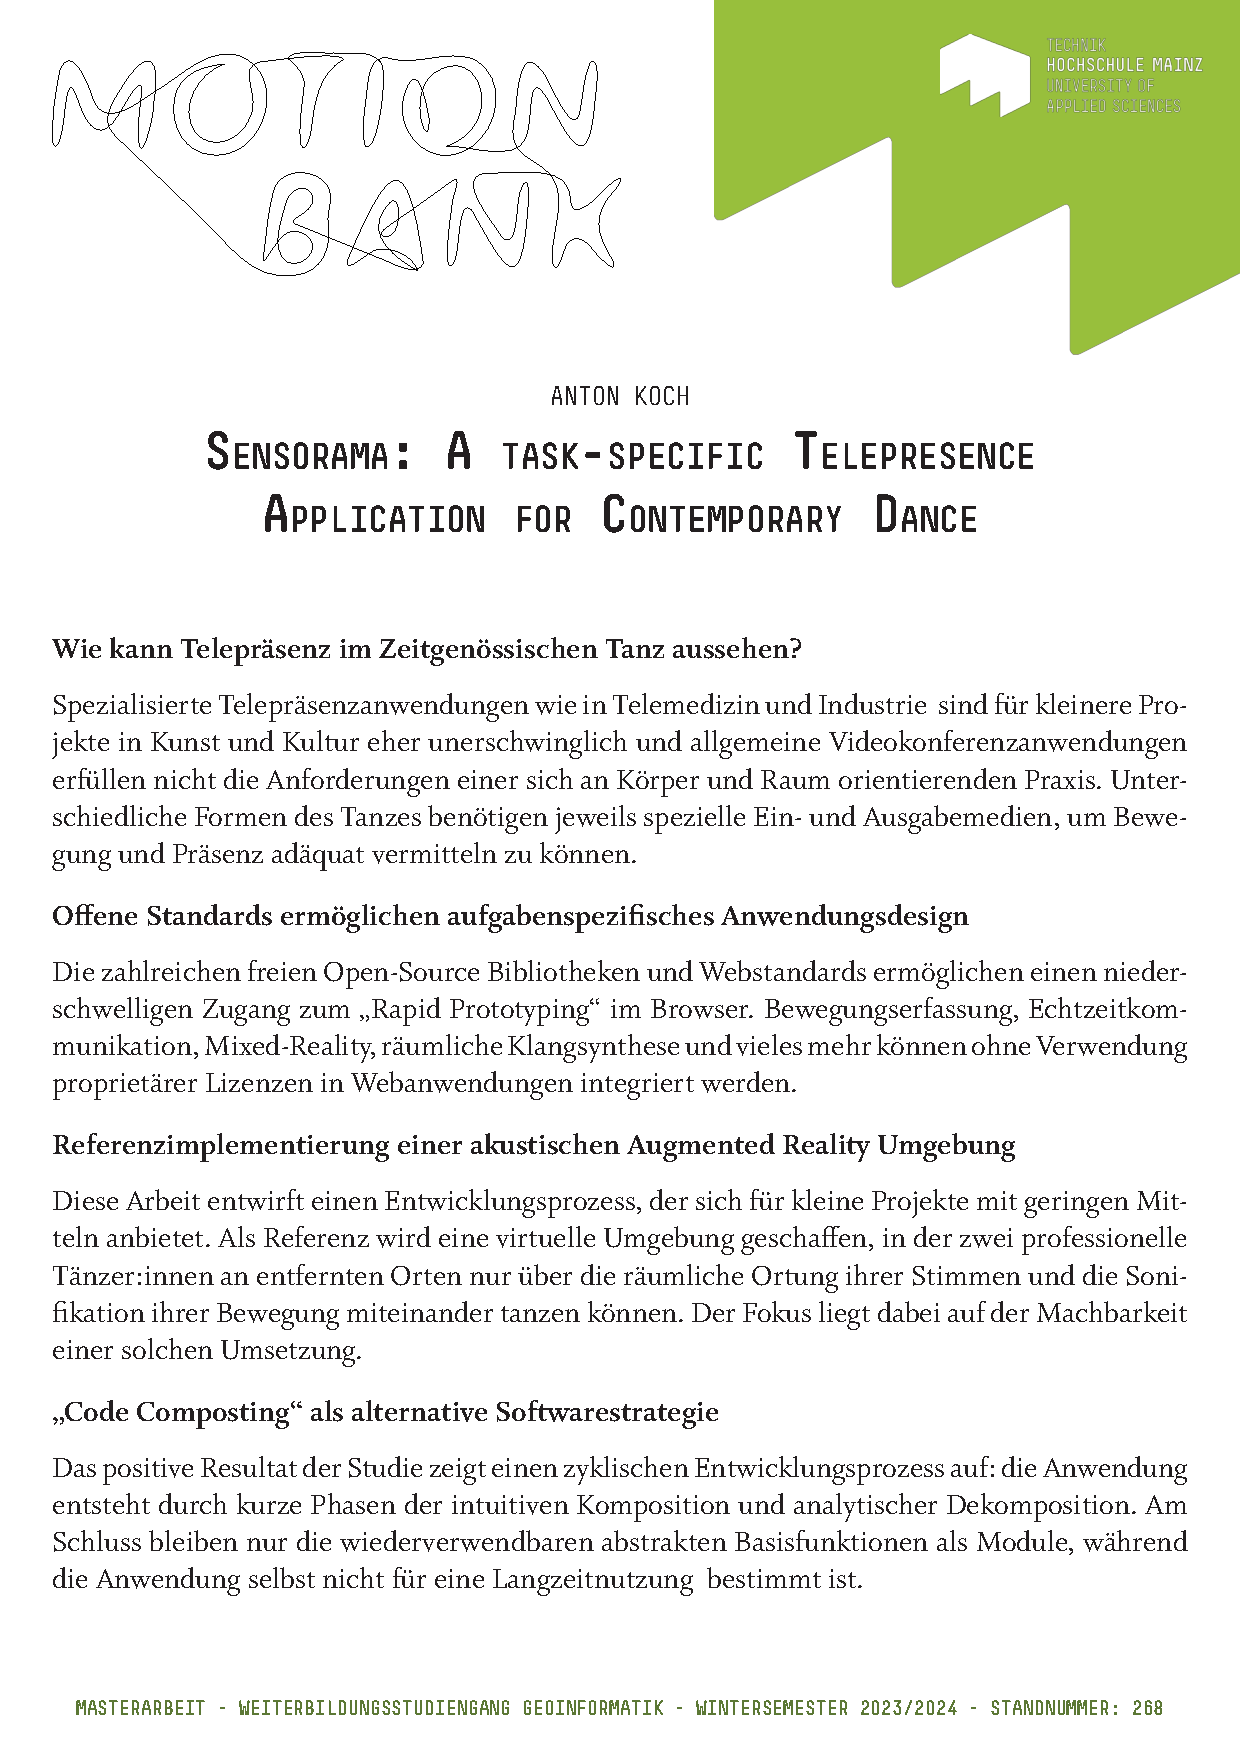
\includegraphics[width=0.7\linewidth]{04_Artefakte/AKoch-Sensorama_Poster-A4.pdf}}
\end{figure}
%
%\chapter{Anhang Tabelle}
%\label{app:longtable}
%\input{04_Artefakte/02_Tabellen/LongSample}


\usestandardtocs
\bookmarksetup{startatroot}% siehe bookmark-Anleitung

\end{document}
